\documentclass[conference]{IEEEtran}
\IEEEoverridecommandlockouts

\usepackage{cite}
\usepackage{amsmath,amssymb,amsfonts}
\usepackage{algorithmic}
\usepackage{graphicx}
\usepackage{textcomp}
\usepackage{xcolor}
\usepackage{subcaption}
\usepackage{hyperref}
\usepackage{algorithm}
\usepackage{algpseudocode}

\def\BibTeX{{\rm B\kern-.05em{\sc i\kern-.025em b}\kern-.08em
    T\kern-.1667em\lower.7ex\hbox{E}\kern-.125emX}}
    
\begin{document}

\title{Multi-UAV Source Seeking and Optimization Using Particle Swarm Optimization Variants\\
}

\author{\IEEEauthorblockN{Dikshant}
\IEEEauthorblockA{\textit{Electronics and Communication Engineering} \\
\textit{IIIT - Hyderabad}\\
Email: dikshant.gurudutt@students.iiit.ac.in}
\and
\IEEEauthorblockN{Dr. Harikumar Kandath}
\IEEEauthorblockA{\textit{Robotics Research Center} \\
\textit{IIIT - Hyderabad}\\
Email: harikumar.k@iiit.ac.in}
}

\maketitle

\begin{abstract}
Investigates the performance of various Particle Swarm Optimization (PSO) variants for multi-UAV source seeking and optimization problems. We compare three PSO variants: Standard PSO (SPSO), Acceleration-based PSO (APSO), and Adaptive Random PSO (ARPSO) in both source seeking scenarios and benchmark optimization functions. Our results demonstrate that APSO consistently outperforms other variants in source seeking tasks, particularly in noisy environments, due to its second-order dynamics that provide smoother trajectories and better noise resilience. However, SPSO shows superior performance on most benchmark optimization functions. We also explore four hybrid approaches that combine these PSO variants in different configurations: Particle Hybrid, Sequential Hybrid, Parallel Hybrid, and Adaptive Hybrid. The Particle Hybrid and Parallel Hybrid approaches demonstrate the most promising overall performance, confirming that strategic combinations of PSO variants can enhance optimization capabilities. This provides insights into algorithm selection for UAV applications and suggests directions for further development of hybrid optimization techniques.
\end{abstract}

\begin{IEEEkeywords}
particle swarm optimization, unmanned aerial vehicles, source seeking, optimization, hybrid algorithms, swarm intelligence
\end{IEEEkeywords}

\section{Introduction}
Unmanned Aerial Vehicles (UAVs) have become increasingly important in various applications, including environmental monitoring, search and rescue operations, and surveillance. Multi-UAV systems offer advantages in terms of robustness, efficiency, and coverage compared to single-UAV approaches. However, coordinating multiple UAVs to efficiently locate sources of interest in complex environments remains a challenging problem.

Particle Swarm Optimization (PSO) is a population-based optimization technique inspired by the social behavior of birds flocking or fish schooling. PSO has been widely applied to various optimization problems due to its simplicity, effectiveness, and ease of implementation. In the context of multi-UAV systems, PSO provides a natural framework for coordinating the movement of multiple agents toward an objective.

As per paper \cite{10312321}, we investigates three PSO variants for multi-UAV source seeking and optimization:
\begin{itemize}
    \item Standard PSO (SPSO): The classic first-order PSO algorithm
    \item Acceleration-based PSO (APSO): A second-order variant that uses acceleration as the primary update mechanism
    \item Adaptive Random PSO (ARPSO): A variant that incorporates adaptive parameters and randomness
\end{itemize}

We evaluate these algorithms in two contexts:
\begin{enumerate}
    \item Source seeking: Finding the source of a signal in environments with and without noise
    \item Optimization: Performance on standard benchmark functions from the CEC 2022 competition
\end{enumerate}

Additionally, we explore four hybrid approaches that combine these PSO variants to leverage their complementary strengths:
\begin{itemize}
    \item Particle Hybrid: Different particles within the same swarm use different update rules
    \item Sequential Hybrid: Different algorithms used in sequence
    \item Parallel Hybrid: Multiple algorithms run simultaneously on separate sub-swarms
    \item Adaptive Hybrid: Dynamically switches between algorithms based on performance
\end{itemize}

The remainder of this report is organized as follows: Section II provides background on PSO variants. Section III describes the source seeking problem and presents experimental results. Section IV evaluates the performance of PSO variants on benchmark functions. Section V introduces hybrid approaches and analyzes their performance. Section VI concludes the paper and discusses future work.

\section{PSO Variants}
\subsection{Standard PSO (SPSO)}
Standard PSO is a first-order optimization algorithm that updates particle positions based on their velocity. Each particle's movement is influenced by its own best-known position and the swarm's global best position.

The mathematical formulation of SPSO is as follows:
\begin{equation}
v_i(t+1) = \omega_1 v_i(t) + c_1 r_1(p_i - x_i) + c_2r_2(g-x_i)
\end{equation}
\begin{equation}
x_i(t+1) = x_i(t) + v_i(t+1)
\end{equation}

where:
\begin{itemize}
    \item $v_i(t)$ is the velocity of particle $i$ at time $t$
    \item $x_i(t)$ is the position of particle $i$ at time $t$
    \item $p_i$ is the best position found by particle $i$ so far
    \item $g$ is the global best position found by any particle
    \item $\omega_1$ is the inertia weight
    \item $c_1$ and $c_2$ are acceleration coefficients
    \item $r_1$ and $r_2$ are random values in the range [0,1]
\end{itemize}

SPSO provides a balanced exploration-exploitation trade-off and is widely used as a baseline algorithm in swarm intelligence applications.

\subsection{Acceleration-based PSO (APSO)}
APSO is a second-order variant of PSO that uses acceleration as the primary update mechanism. This approach maintains momentum through previous movement history and produces smoother trajectories with more consistent direction.

The mathematical formulation of APSO is:
\begin{equation}
a_i(t+1) = \omega_1 a_i(t) + c_1 r_1(p_i - x_i) + c_2r_2(g-x_i)
\end{equation}
\begin{equation}
v_i(t+1) = \omega_2v_i(t) + a_i(t+1)T
\end{equation}
\begin{equation}
x_i(t+1) = x_i(t) + v_i(t+1)T
\end{equation}

where:
\begin{itemize}
    \item $a_i(t)$ is the acceleration of particle $i$ at time $t$
    \item $T$ is the time step
    \item $\omega_2$ is the velocity damping coefficient
\end{itemize}

The second-order dynamics of APSO allow it to maintain momentum, which can be beneficial in noisy environments where consistent movement direction is important.

\subsection{Adaptive Random PSO (ARPSO)}
ARPSO incorporates adaptive parameters and randomness to enhance exploration capabilities. It dynamically adjusts the inertia weight based on the swarm's state and includes additional random attractive positions to help particles escape local optima.

The mathematical formulation of ARPSO is:
\begin{equation}
\omega_i(t+1) = f(\text{evolutionary speed}, \text{aggregation degree})
\end{equation}
\begin{equation}
v_i(t+1) = \omega_iv_i(t) + c_1r_1(p_i-x_i) + c_2r_2(g-x_i) + c_3r_3(a_i-x_i)
\end{equation}
\begin{equation}
x_i(t+1) = x_i(t) + v_i(t+1)
\end{equation}

where:
\begin{itemize}
    \item $\omega_i(t)$ is the adaptive inertia weight for particle $i$ at time $t$
    \item $a_i$ is a random attractive position
    \item $c_3$ is the coefficient for the random attraction
    \item $r_3$ is a random value in the range [0,1]
\end{itemize}

The adaptive inertia weight is adjusted based on:
\begin{itemize}
    \item Evolutionary speed: How quickly the swarm's best solution is improving
    \item Aggregation degree: How clustered the particles are in the search space
\end{itemize}

When particles cluster too much (high aggregation), the inertia weight increases to push particles to explore more widely. When improvement slows down, the inertia weight is adjusted to help escape potential local optima.

\section{Source Seeking}
\subsection{Problem Formulation}
The source seeking problem involves finding the location of a signal source in an environment. The signal strength typically follows a distribution that decreases with distance from the source. In our experiments, we use a Gaussian distribution centered at the source location:

\begin{equation}
S(x,y) = A \cdot \exp\left(-\frac{(x-x_s)^2 + (y-y_s)^2}{2\sigma^2}\right)
\end{equation}

where:
\begin{itemize}
    \item $S(x,y)$ is the signal strength at position $(x,y)$
    \item $(x_s, y_s)$ is the source location
    \item $A$ is the maximum signal strength
    \item $\sigma$ is the spread parameter
\end{itemize}

In noisy environments, the measured signal strength includes additive noise:

\begin{equation}
S_{measured}(x,y) = S(x,y) + \eta
\end{equation}

where $\eta$ is Gaussian noise with zero mean and standard deviation proportional to the noise level.

\subsection{Experimental Setup}
We conducted experiments to evaluate the performance of SPSO, APSO, and ARPSO in source-seeking tasks with and without noise. The experimental parameters were:

\begin{itemize}
    \item Search space: 100m × 100m
    \item Source location: Randomly placed within the search space
    \item Number of UAVs: 5 to 30
    \item Noise levels: 0 to 0.15 (as a fraction of maximum signal strength)
    \item Convergence criterion: Global best position within 2m of the source
    \item Number of runs: 5 for each configuration
\end{itemize}

Performance metrics included:
\begin{itemize}
    \item Number of iterations to convergence
    \item Total distance traveled by all UAVs
\end{itemize}

\subsection{Results without Noise}
Fig. 1 shows the performance of the three PSO variants in source seeking without noise as the number of UAVs increases.

\begin{figure}[htbp]
\centering
\begin{subfigure}{0.49\linewidth}
    \centering
    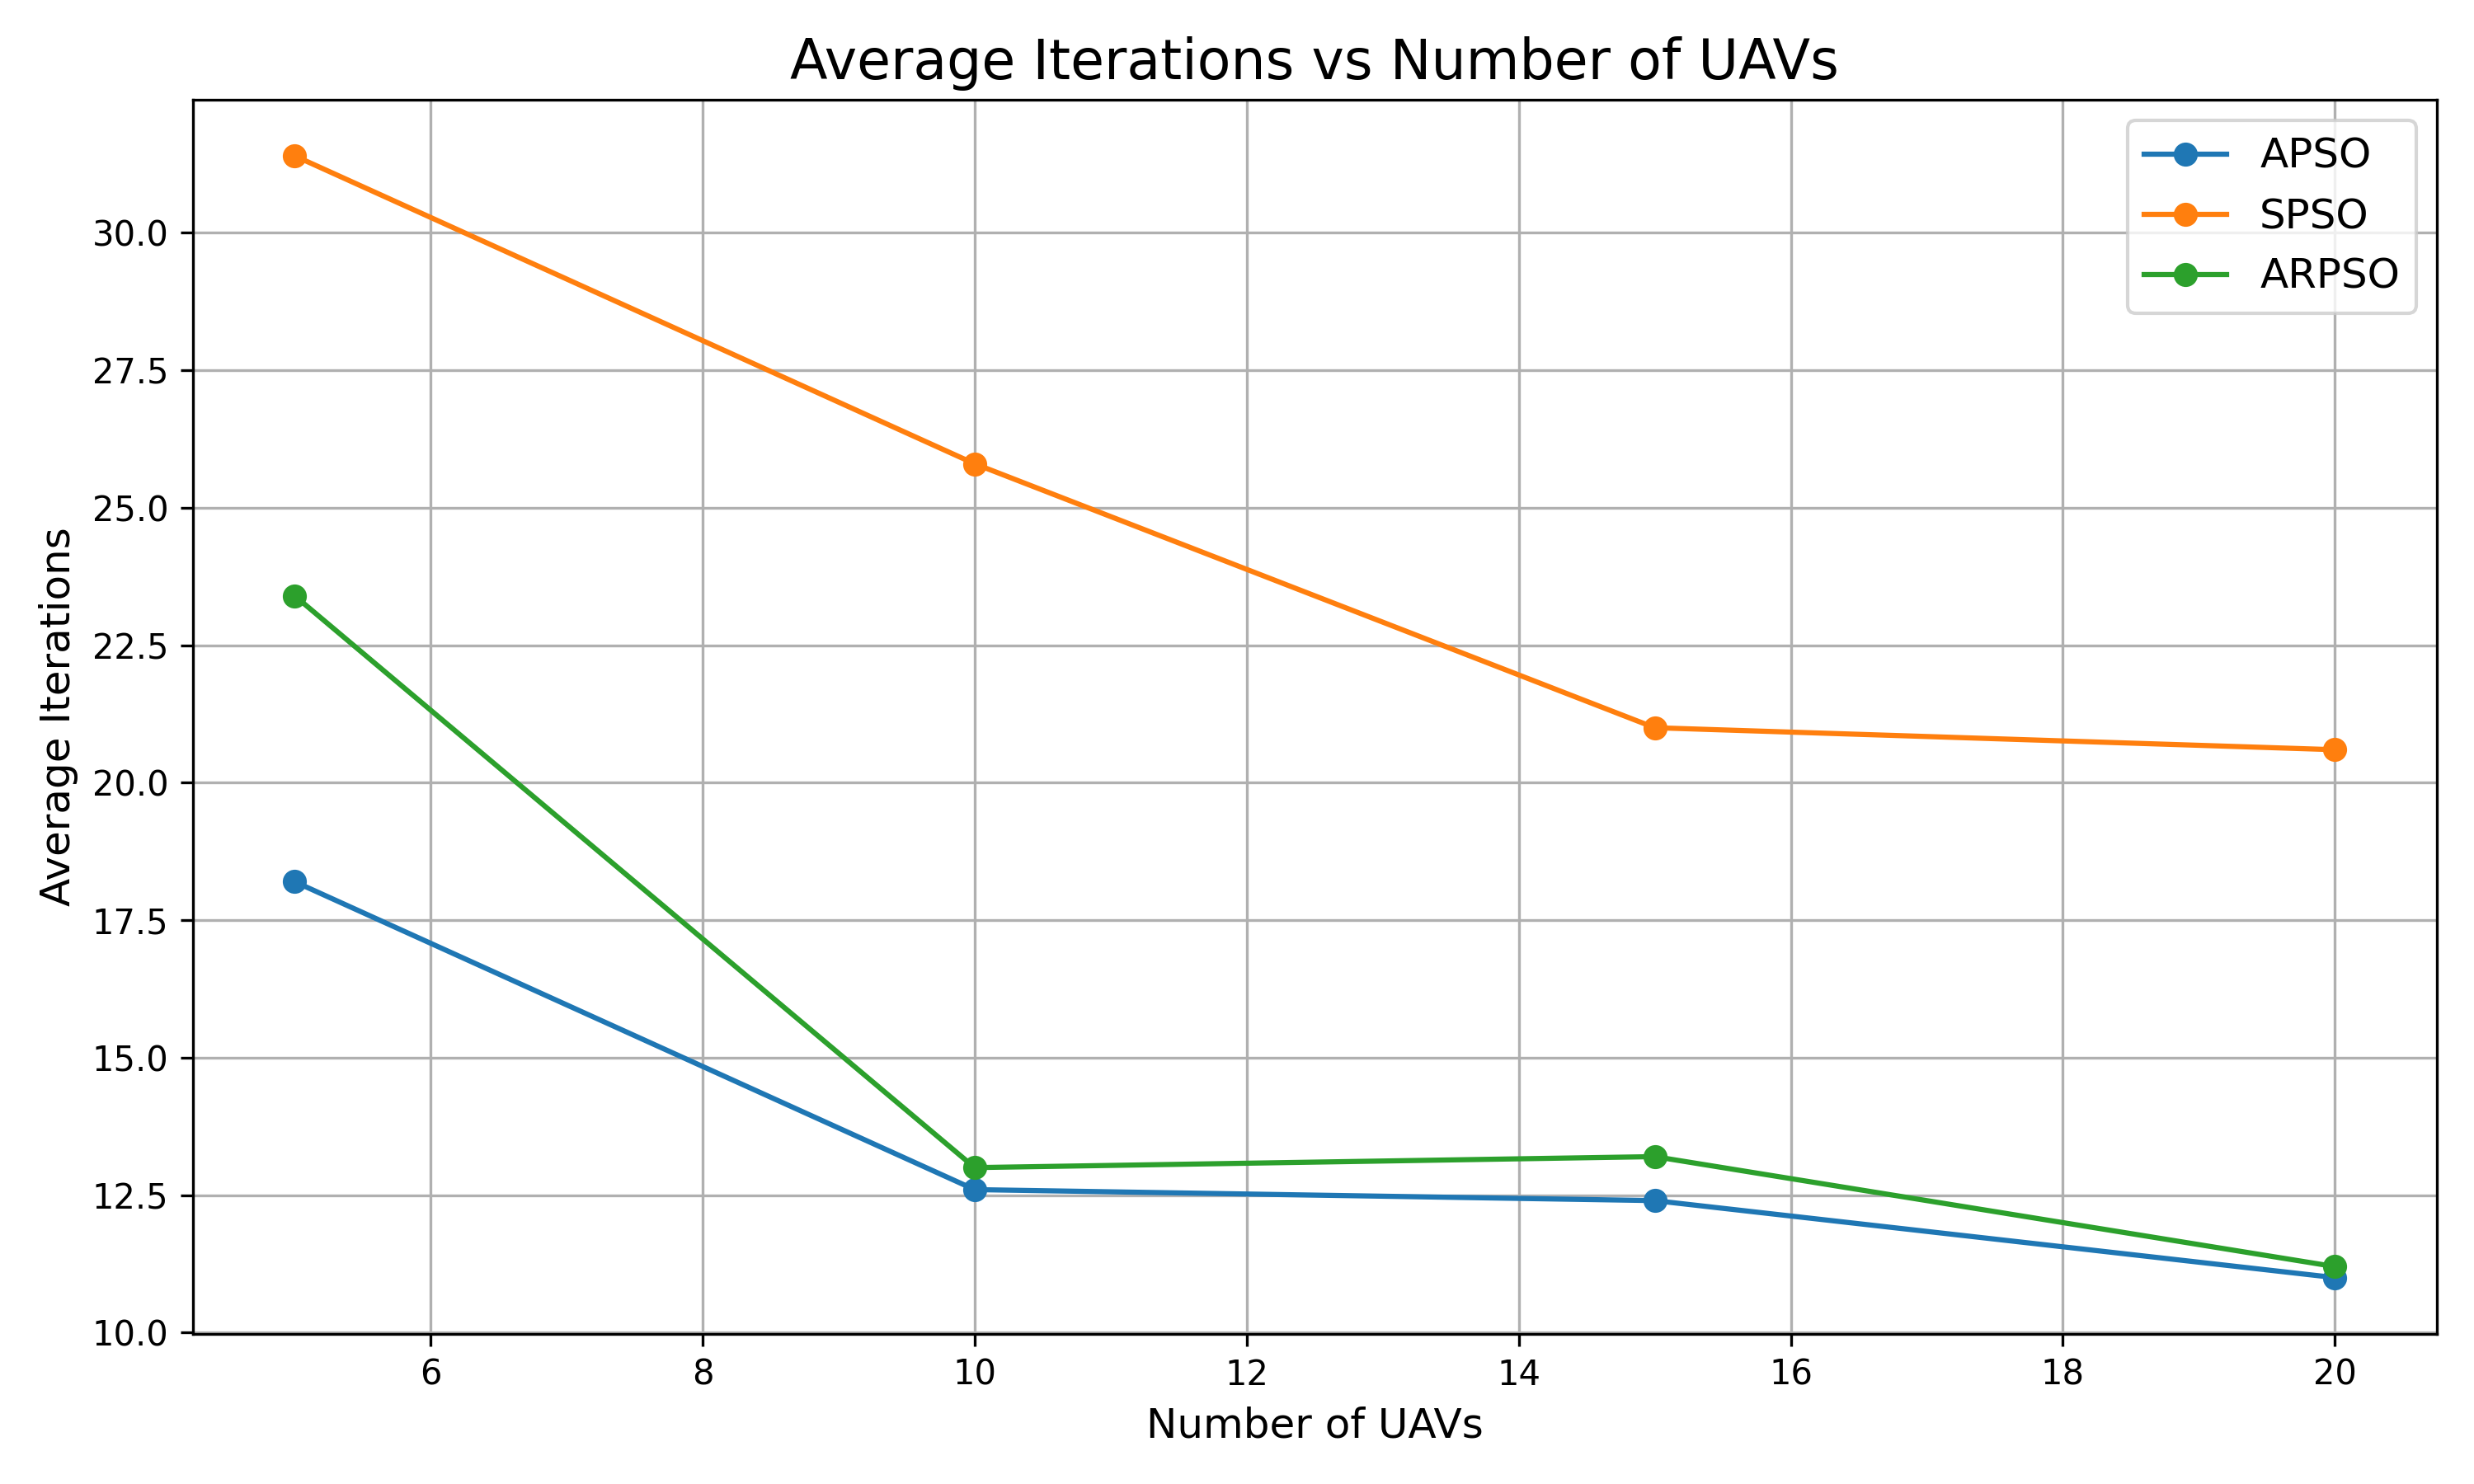
\includegraphics[width=\linewidth]{../plots/r2_without_noise/iterations_vs_#UAVs.png}
    \caption{Iterations vs. Number of UAVs}
    \label{fig:iterations_vs_uavs}
\end{subfigure}
\hfill
\begin{subfigure}{0.49\linewidth}
    \centering
    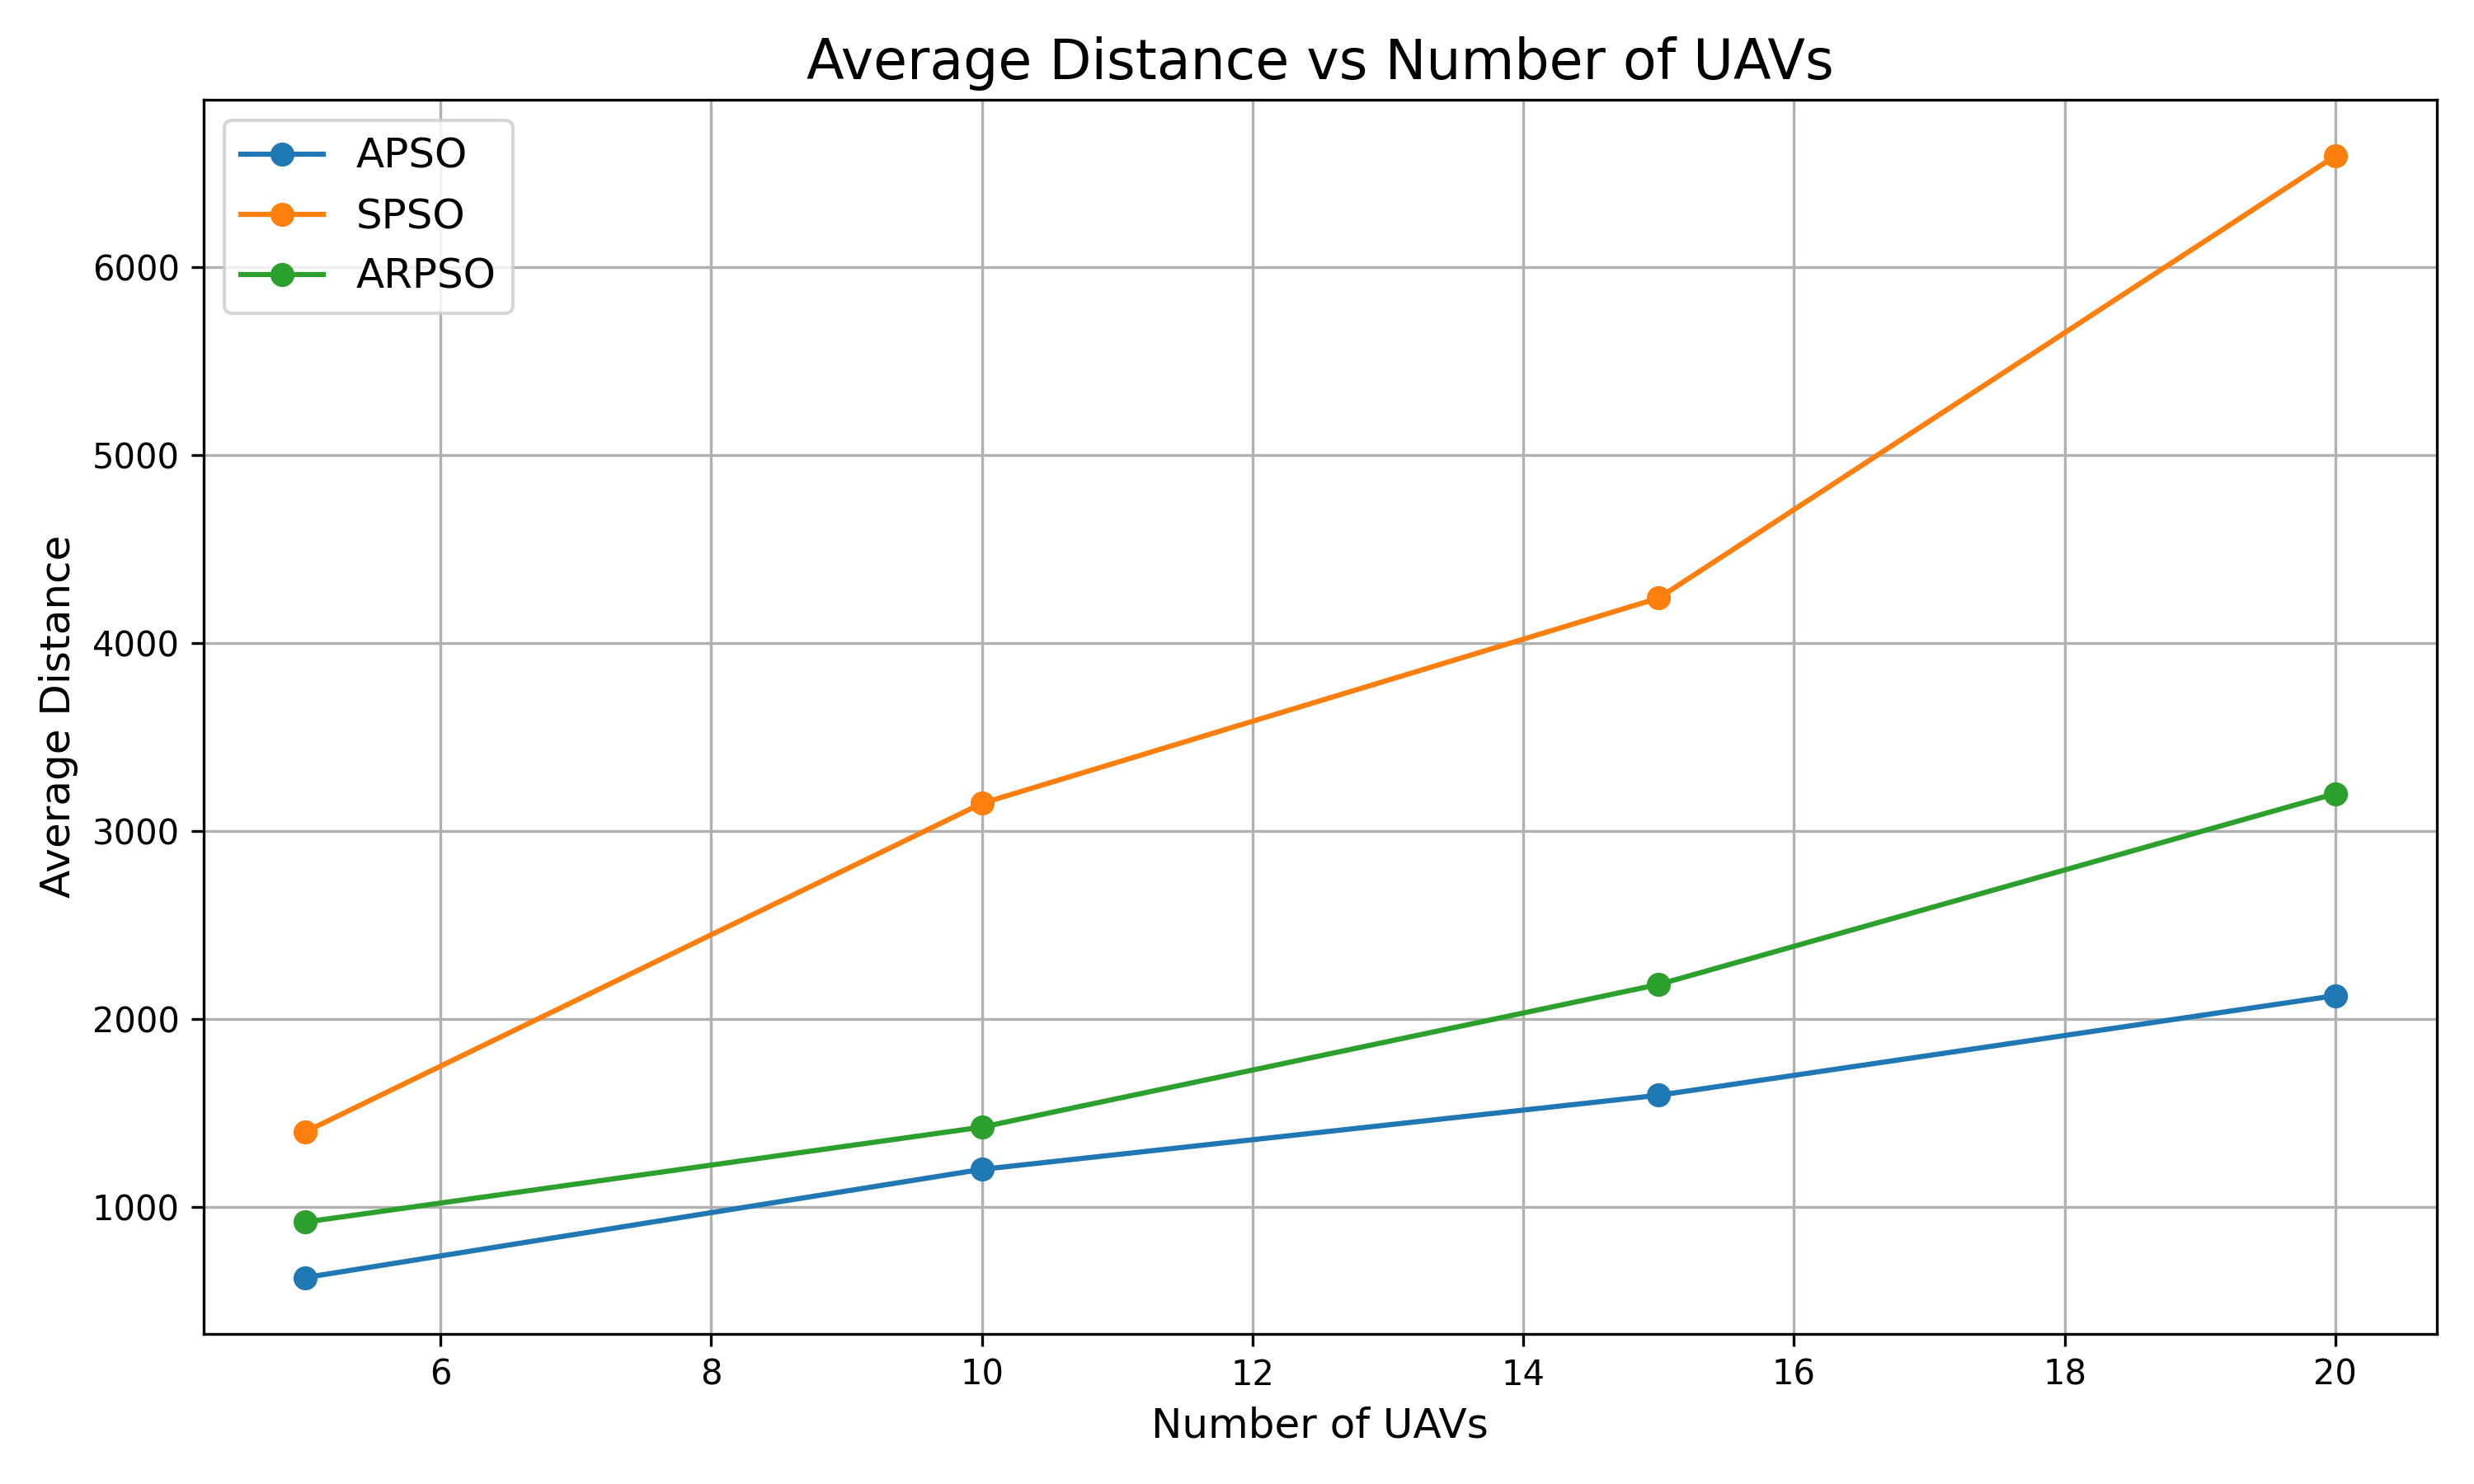
\includegraphics[width=\linewidth]{../plots/r2_without_noise/distance_vs_#UAVs.png}
    \caption{Distance vs. Number of UAVs}
    \label{fig:distance_vs_uavs}
\end{subfigure}
\caption{Source seeking performance without noise}
\label{fig:source_seeking_no_noise}
\end{figure}

Key observations:
\begin{itemize}
    \item APSO consistently outperforms both SPSO and ARPSO in terms of iterations and distance traveled
    \item APSO shows the best scaling as UAV count increases, with iterations actually decreasing as more UAVs are added
    \item SPSO shows the worst scaling in terms of distance traveled
\end{itemize}

\subsection{Results with Noise}
Fig. 2 shows the performance of the three PSO variants in source seeking with varying noise levels for 30 UAVs.

\begin{figure}[htbp]
\centering
\begin{subfigure}{0.49\linewidth}
    \centering
    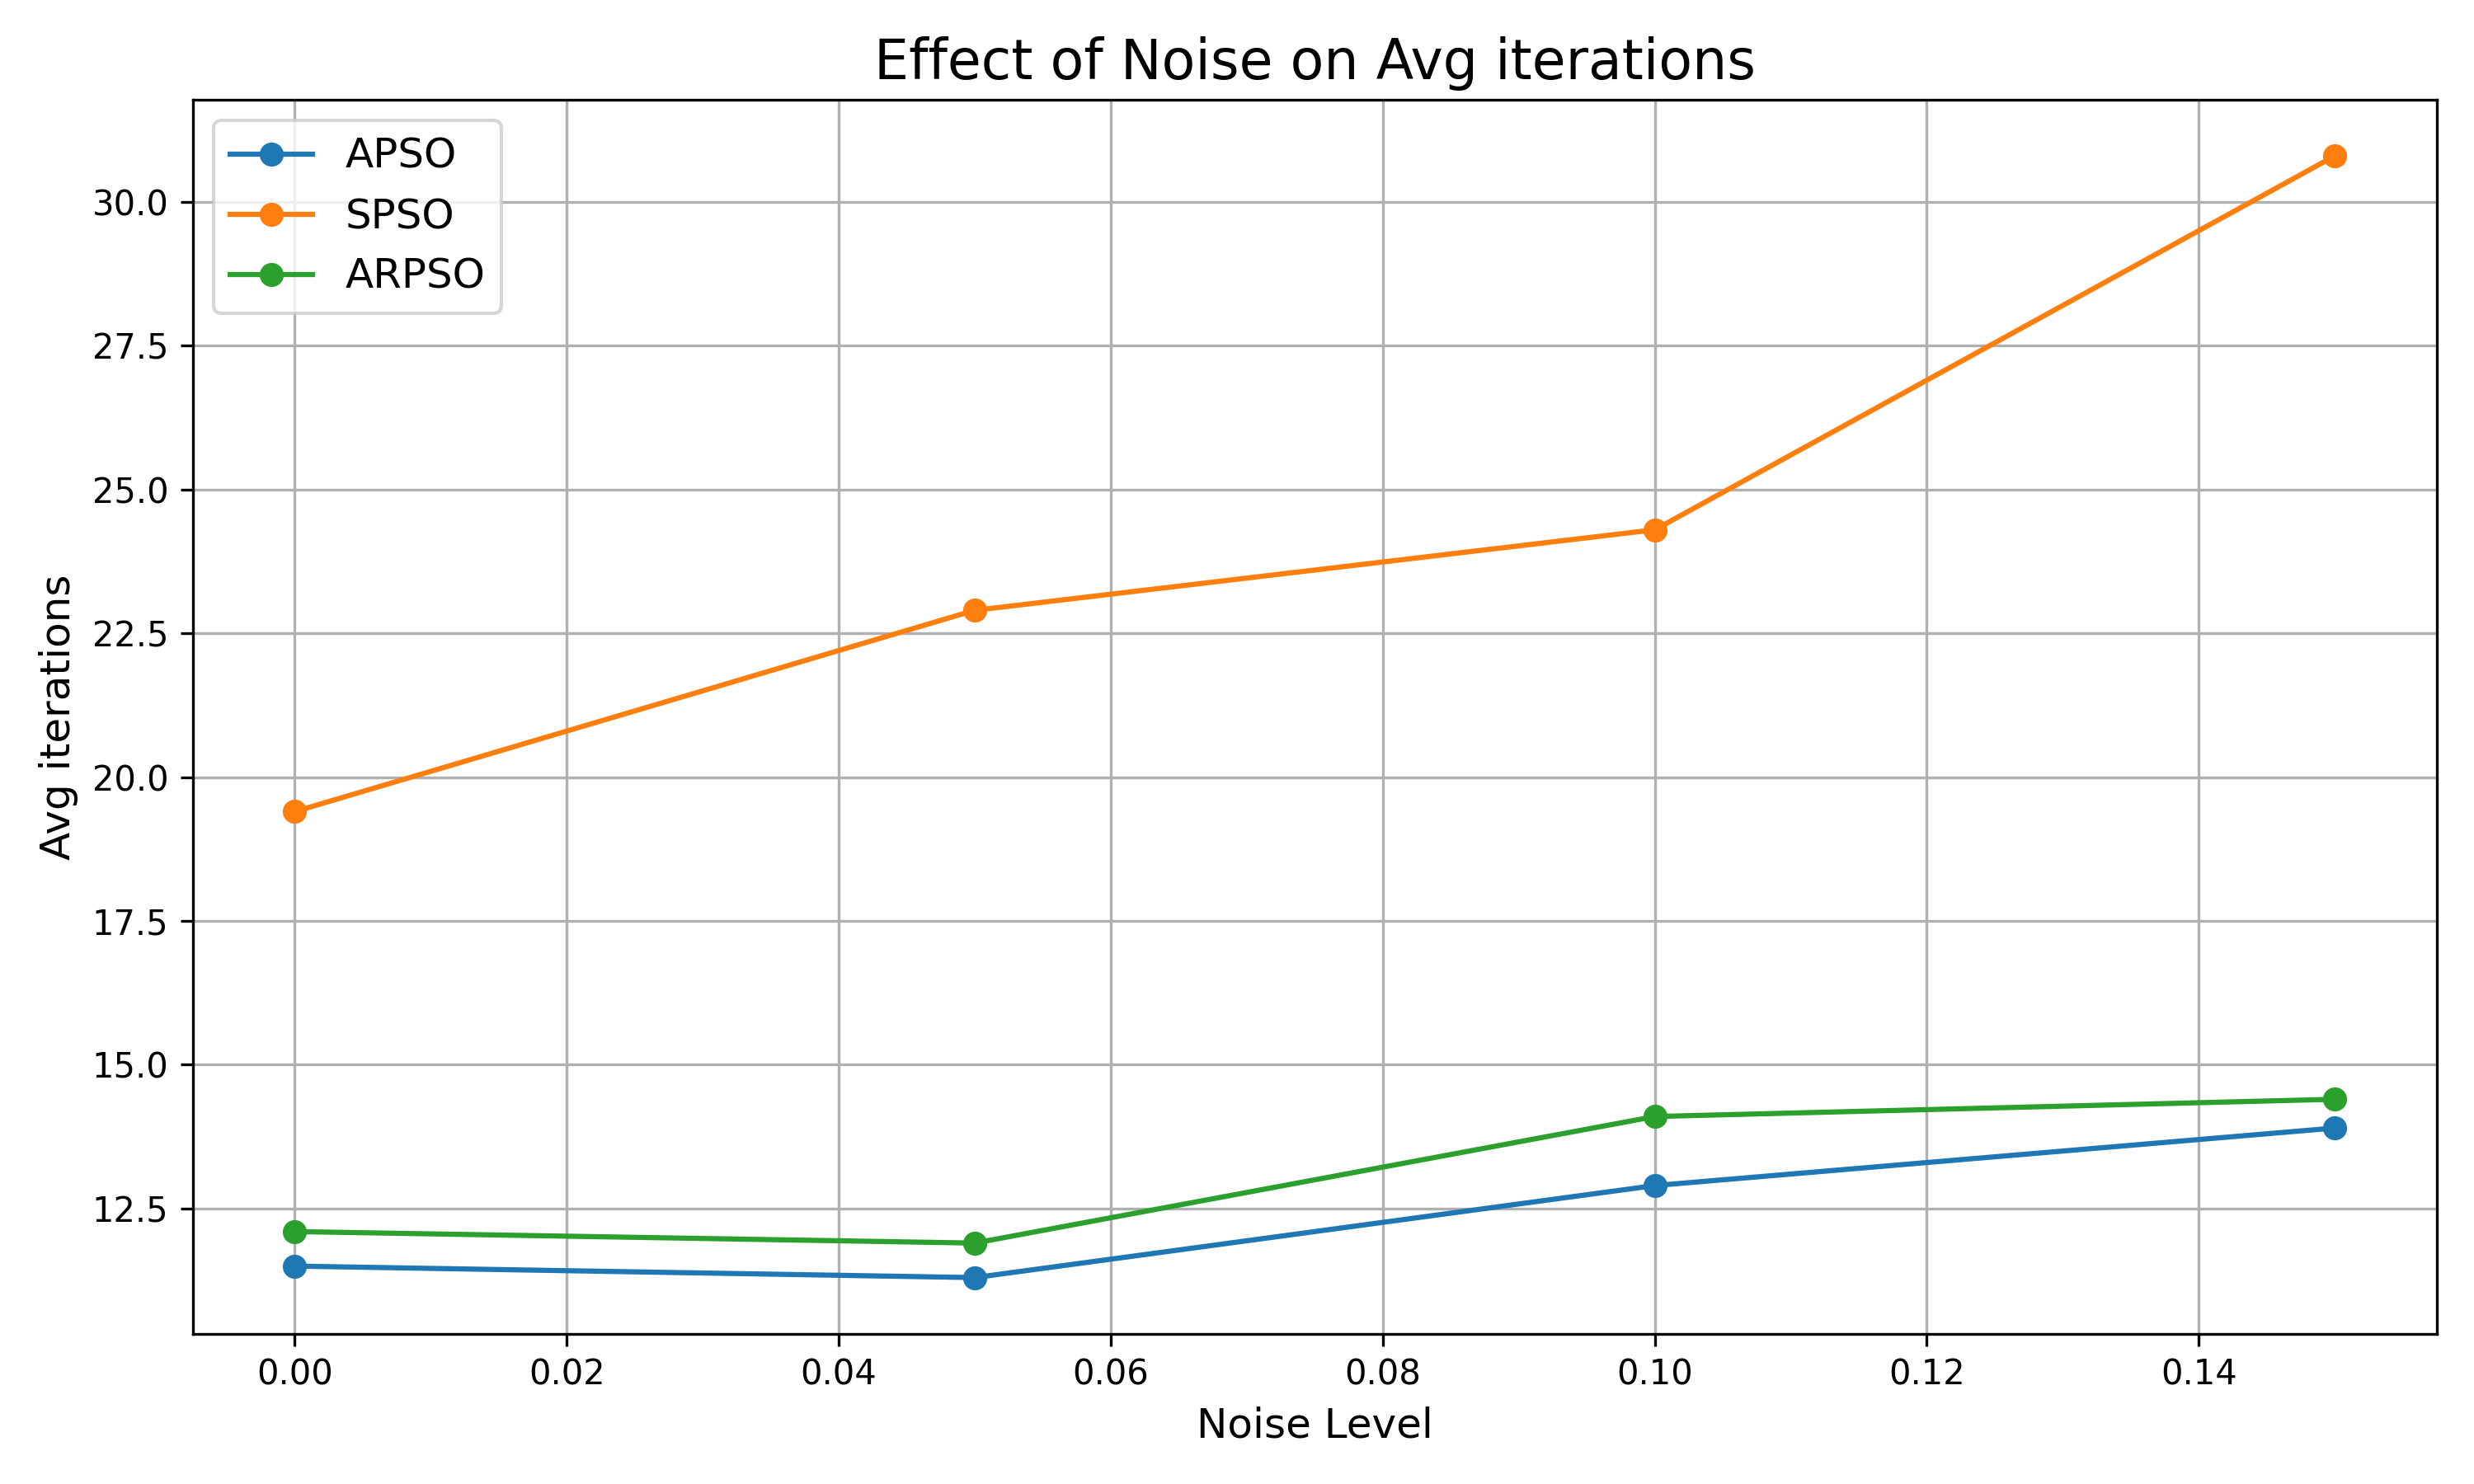
\includegraphics[width=\linewidth]{../plots/r1_with_noise/avg_iterations_vs_noise.png}
    \caption{Iterations vs. Noise Level}
    \label{fig:iterations_vs_noise}
\end{subfigure}
\hfill
\begin{subfigure}{0.49\linewidth}
    \centering
    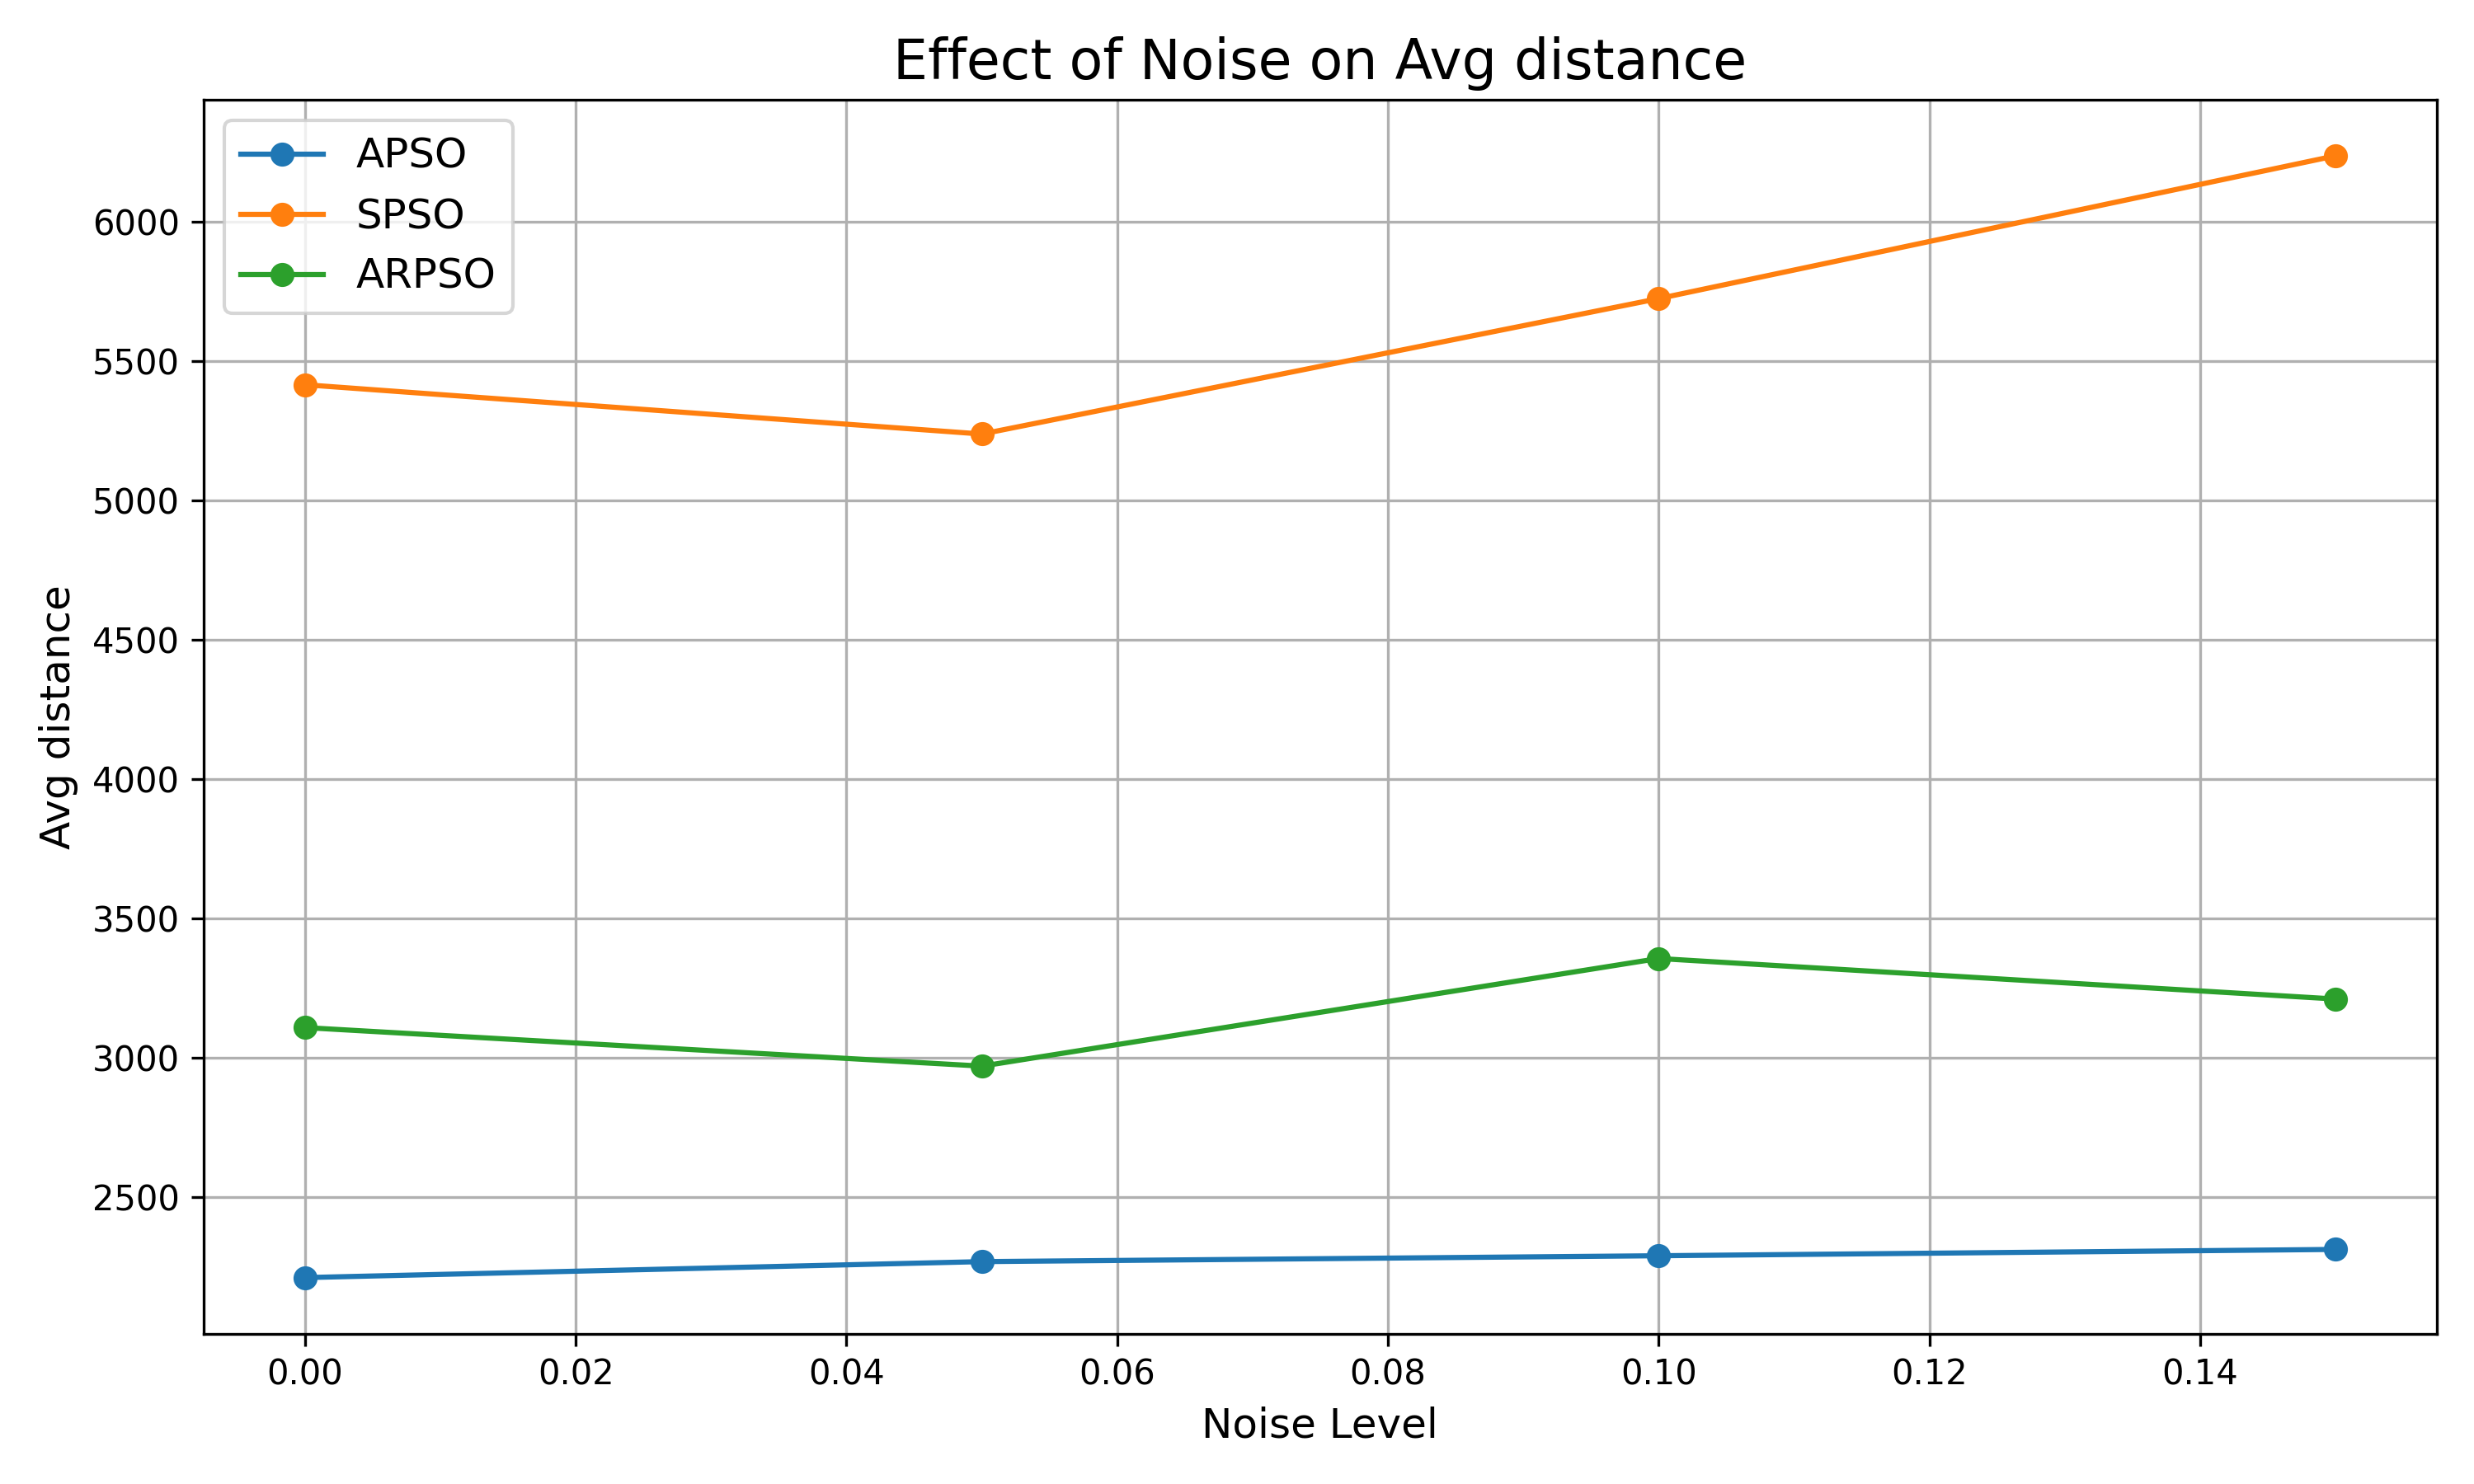
\includegraphics[width=\linewidth]{../plots/r1_with_noise/avg_distance_vs_noise.png}
    \caption{Distance vs. Noise Level}
    \label{fig:distance_vs_noise}
\end{subfigure}
\caption{Source seeking performance with noise (30 UAVs)}
\label{fig:source_seeking_with_noise}
\end{figure}

Key observations:
\begin{itemize}
    \item All algorithms show degraded performance as noise increases
    \item APSO maintains the best performance across all noise levels
    \item APSO shows the best robustness to noise, with a less steep performance degradation
    \item Even at 0.15 noise level, APSO maintains good performance
\end{itemize}

\subsection{Discussion}
APSO's superior performance in source seeking can be attributed to its second-order dynamics, which provide several advantages:

\begin{itemize}
    \item Momentum: APSO maintains momentum through previous movement history, making it less susceptible to being misled by noisy measurements
    \item Smooth trajectories: The acceleration-based approach produces smoother trajectories that are more energy-efficient for UAVs
    \item Noise filtering: The second-order dynamics naturally filter out noise through momentum
    \item Consistent direction: APSO maintains more consistent movement direction, which is beneficial when navigating toward a source
\end{itemize}

The decreasing number of iterations with increasing UAV count for APSO is particularly interesting. This suggests that APSO effectively leverages the parallel exploration capability of multiple UAVs, with more UAVs providing better sampling of the environment and faster convergence.

\section{Benchmark Function Optimization}
\subsection{CEC 2022 Benchmark Functions}
To evaluate the optimization performance of the PSO variants, we used five functions from the CEC 2022 benchmark suite \cite{luo2022benchmarkfunctionscec2022}:

\begin{itemize}
    \item F1 (Zakharov): Continuous unimodal function with interdependent variables
    \item F2 (Rosenbrock): Continuous function with narrow curved valley
    \item F3 (Schaffer): Highly multimodal function with many local optima
    \item F4 (Step Rastrigin): Discontinuous multimodal function with plateaus
    \item F5 (Levy): Multimodal function with many local minima
\end{itemize}

These functions represent diverse optimization challenges:
\begin{itemize}
    \item F1-F2: Test convergence precision and speed
    \item F3-F5: Test ability to escape local optima
\end{itemize}

\subsection{Experimental Setup}
We conducted experiments with the following parameters:
\begin{itemize}
    \item Dimension: 10
    \item Number of particles: 30
    \item Maximum iterations: 200
    \item Number of runs: 5 for each function and algorithm
\end{itemize}

Performance was measured by the final function value achieved (lower is better).

\subsection{Results}
Fig. 3 shows the convergence behavior of the three PSO variants on the five benchmark functions.

\begin{figure}[htbp]
\centering
\begin{subfigure}{0.32\linewidth}
    \centering
    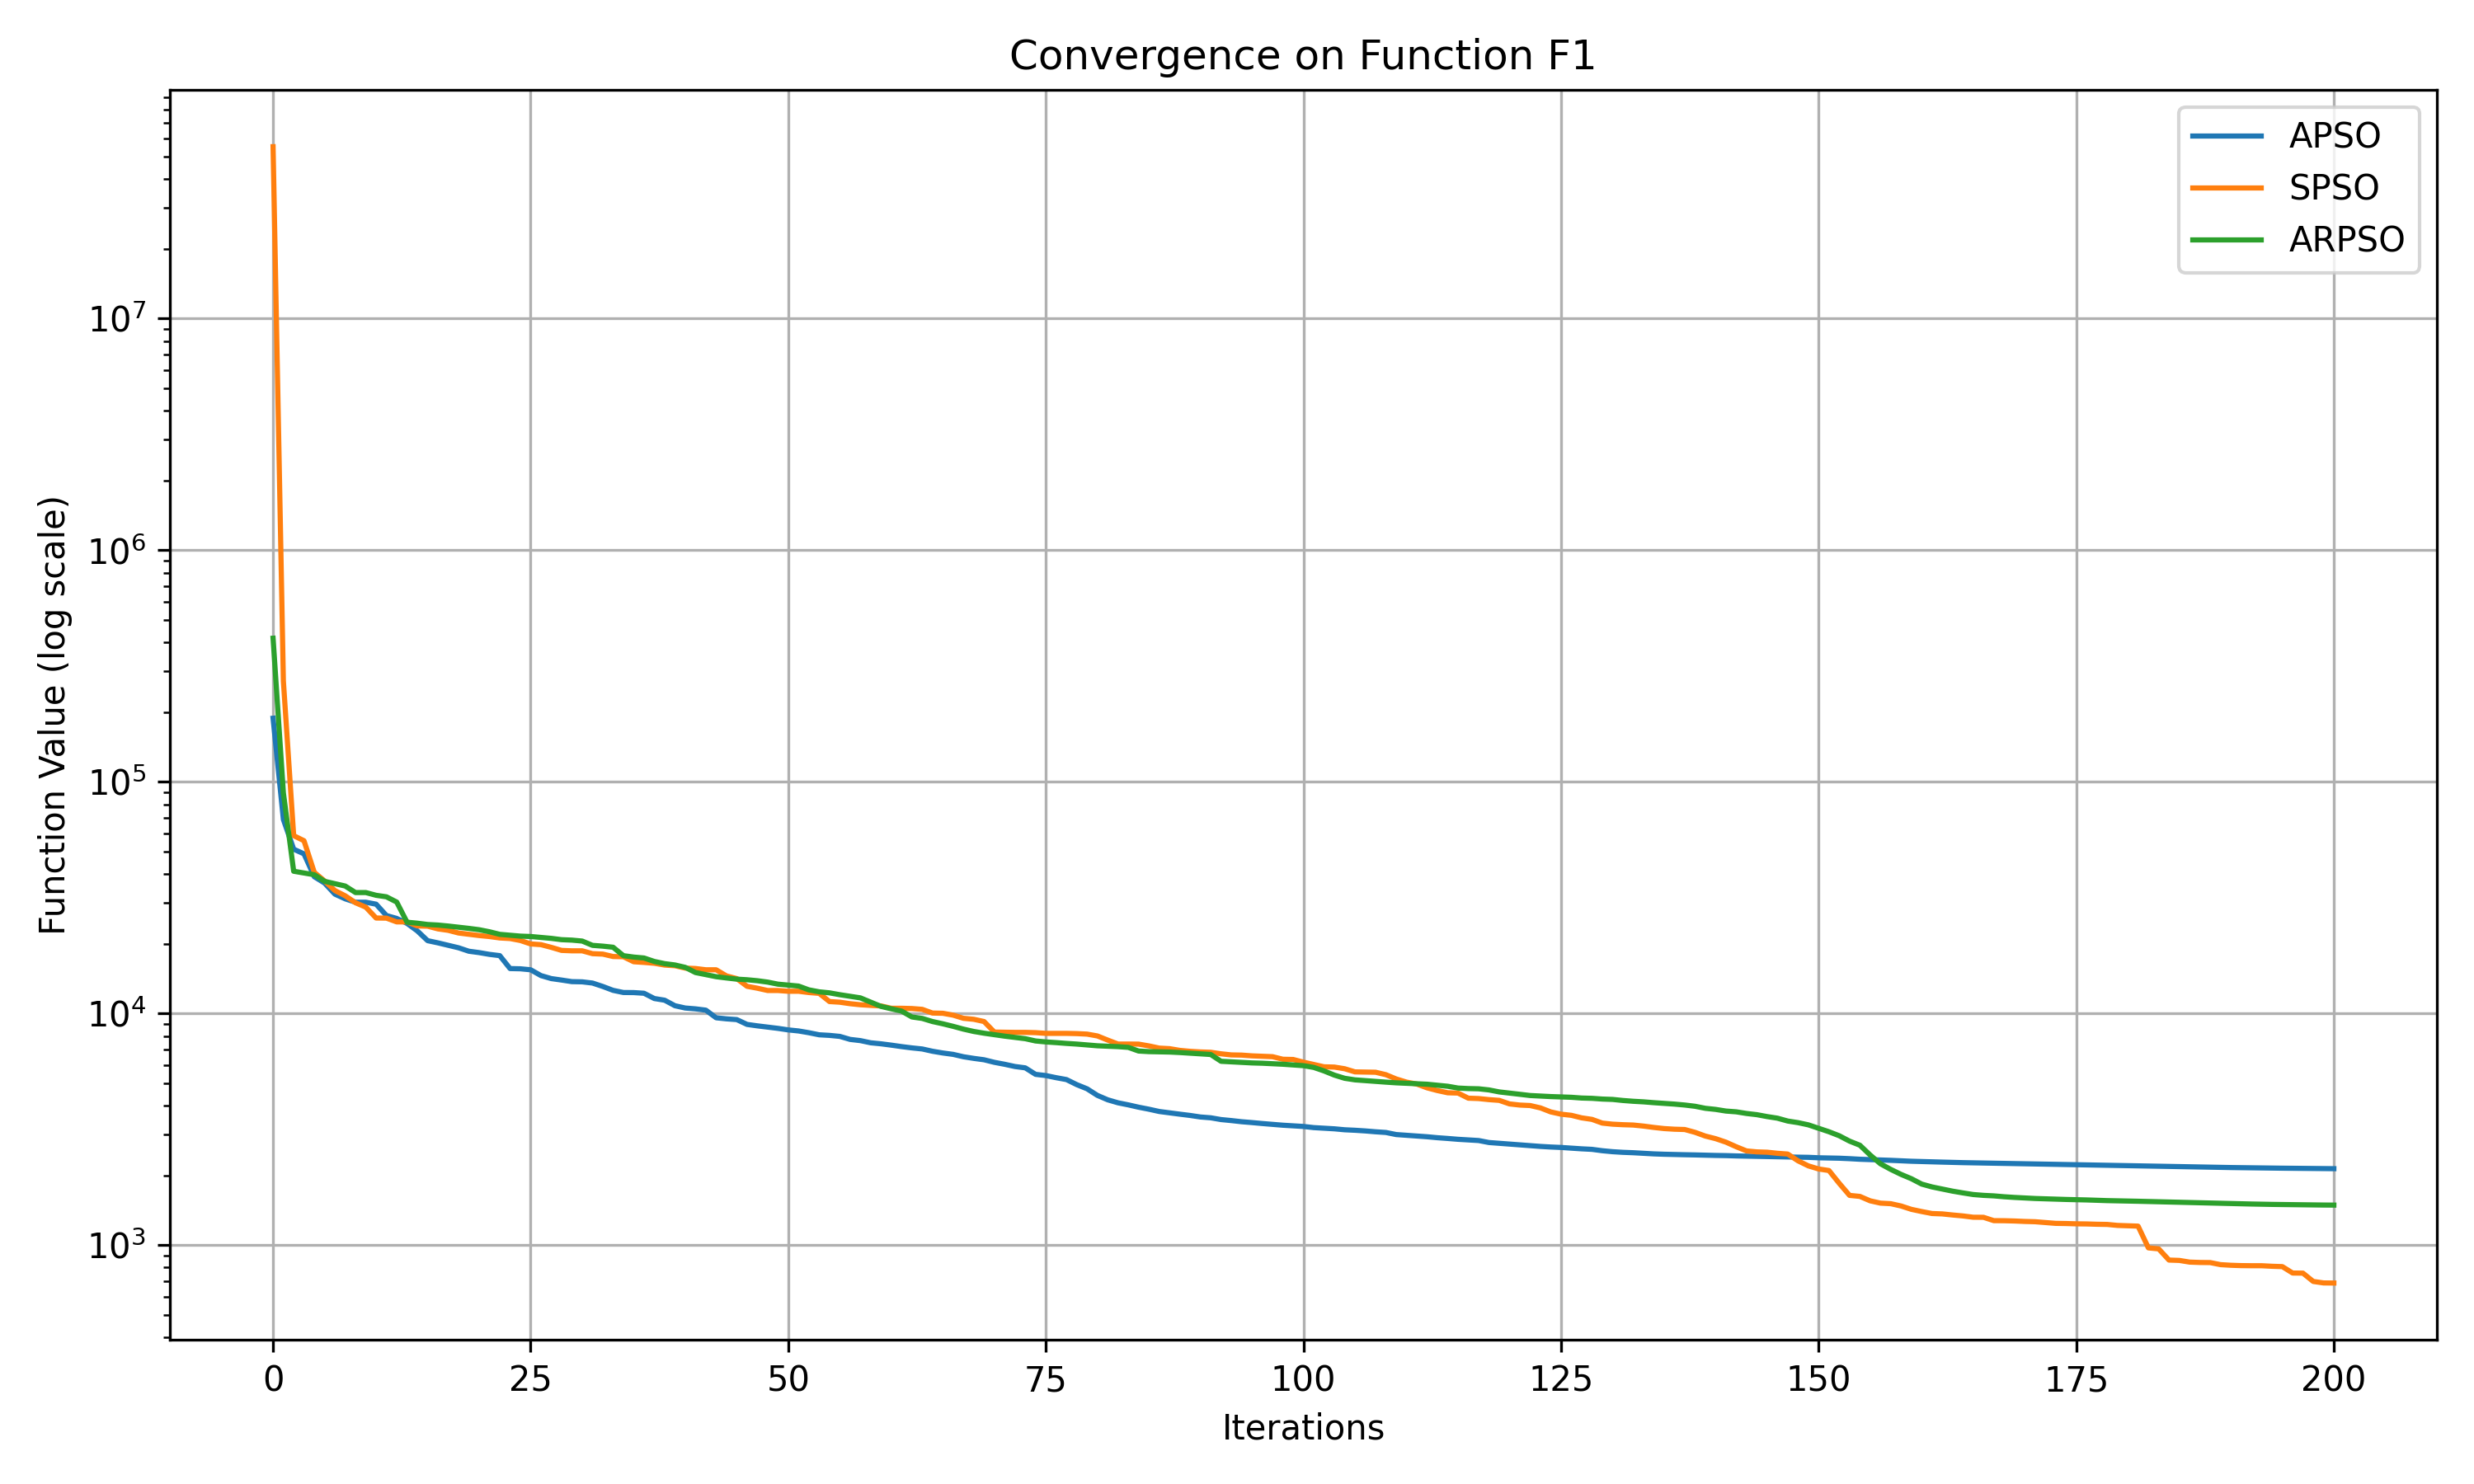
\includegraphics[width=\linewidth]{../plots/cec_bench/cec_convergence_f1.png}
    \caption{F1 (Zakharov)}
    \label{fig:conv_f1}
\end{subfigure}
\hfill
\begin{subfigure}{0.32\linewidth}
    \centering
    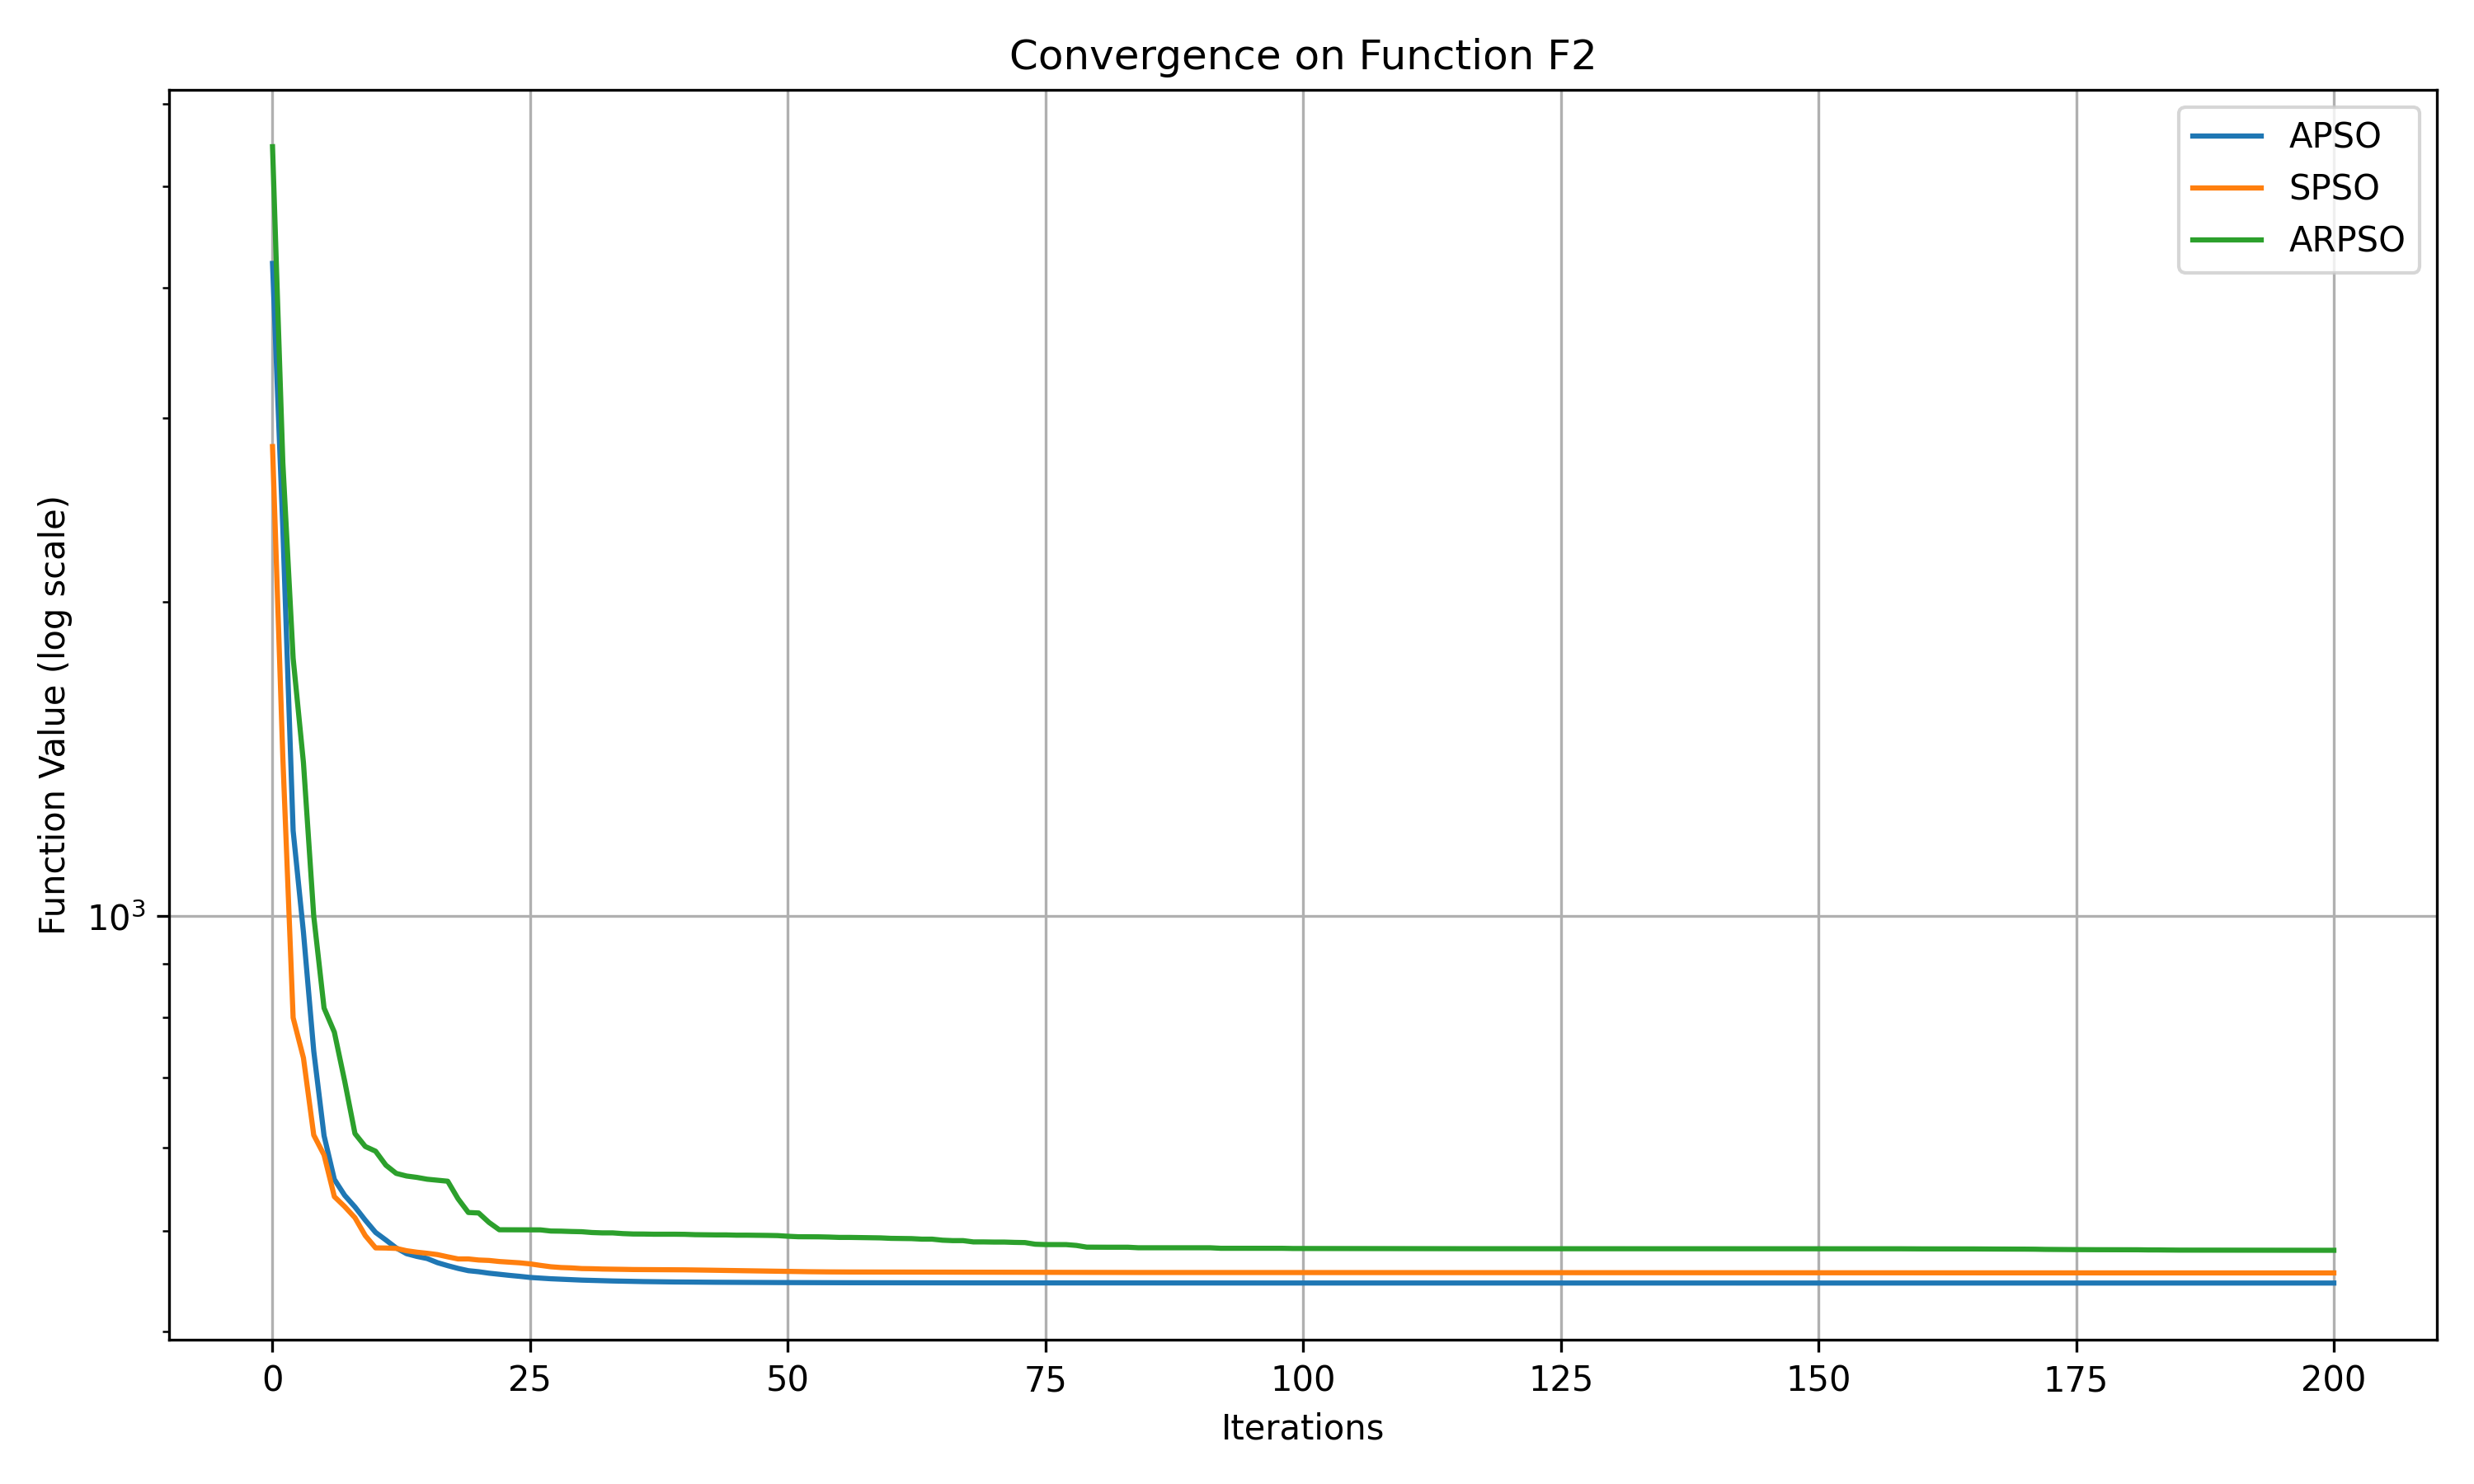
\includegraphics[width=\linewidth]{../plots/cec_bench/cec_convergence_f2.png}
    \caption{F2 (Rosenbrock)}
    \label{fig:conv_f2}
\end{subfigure}
\hfill
\begin{subfigure}{0.32\linewidth}
    \centering
    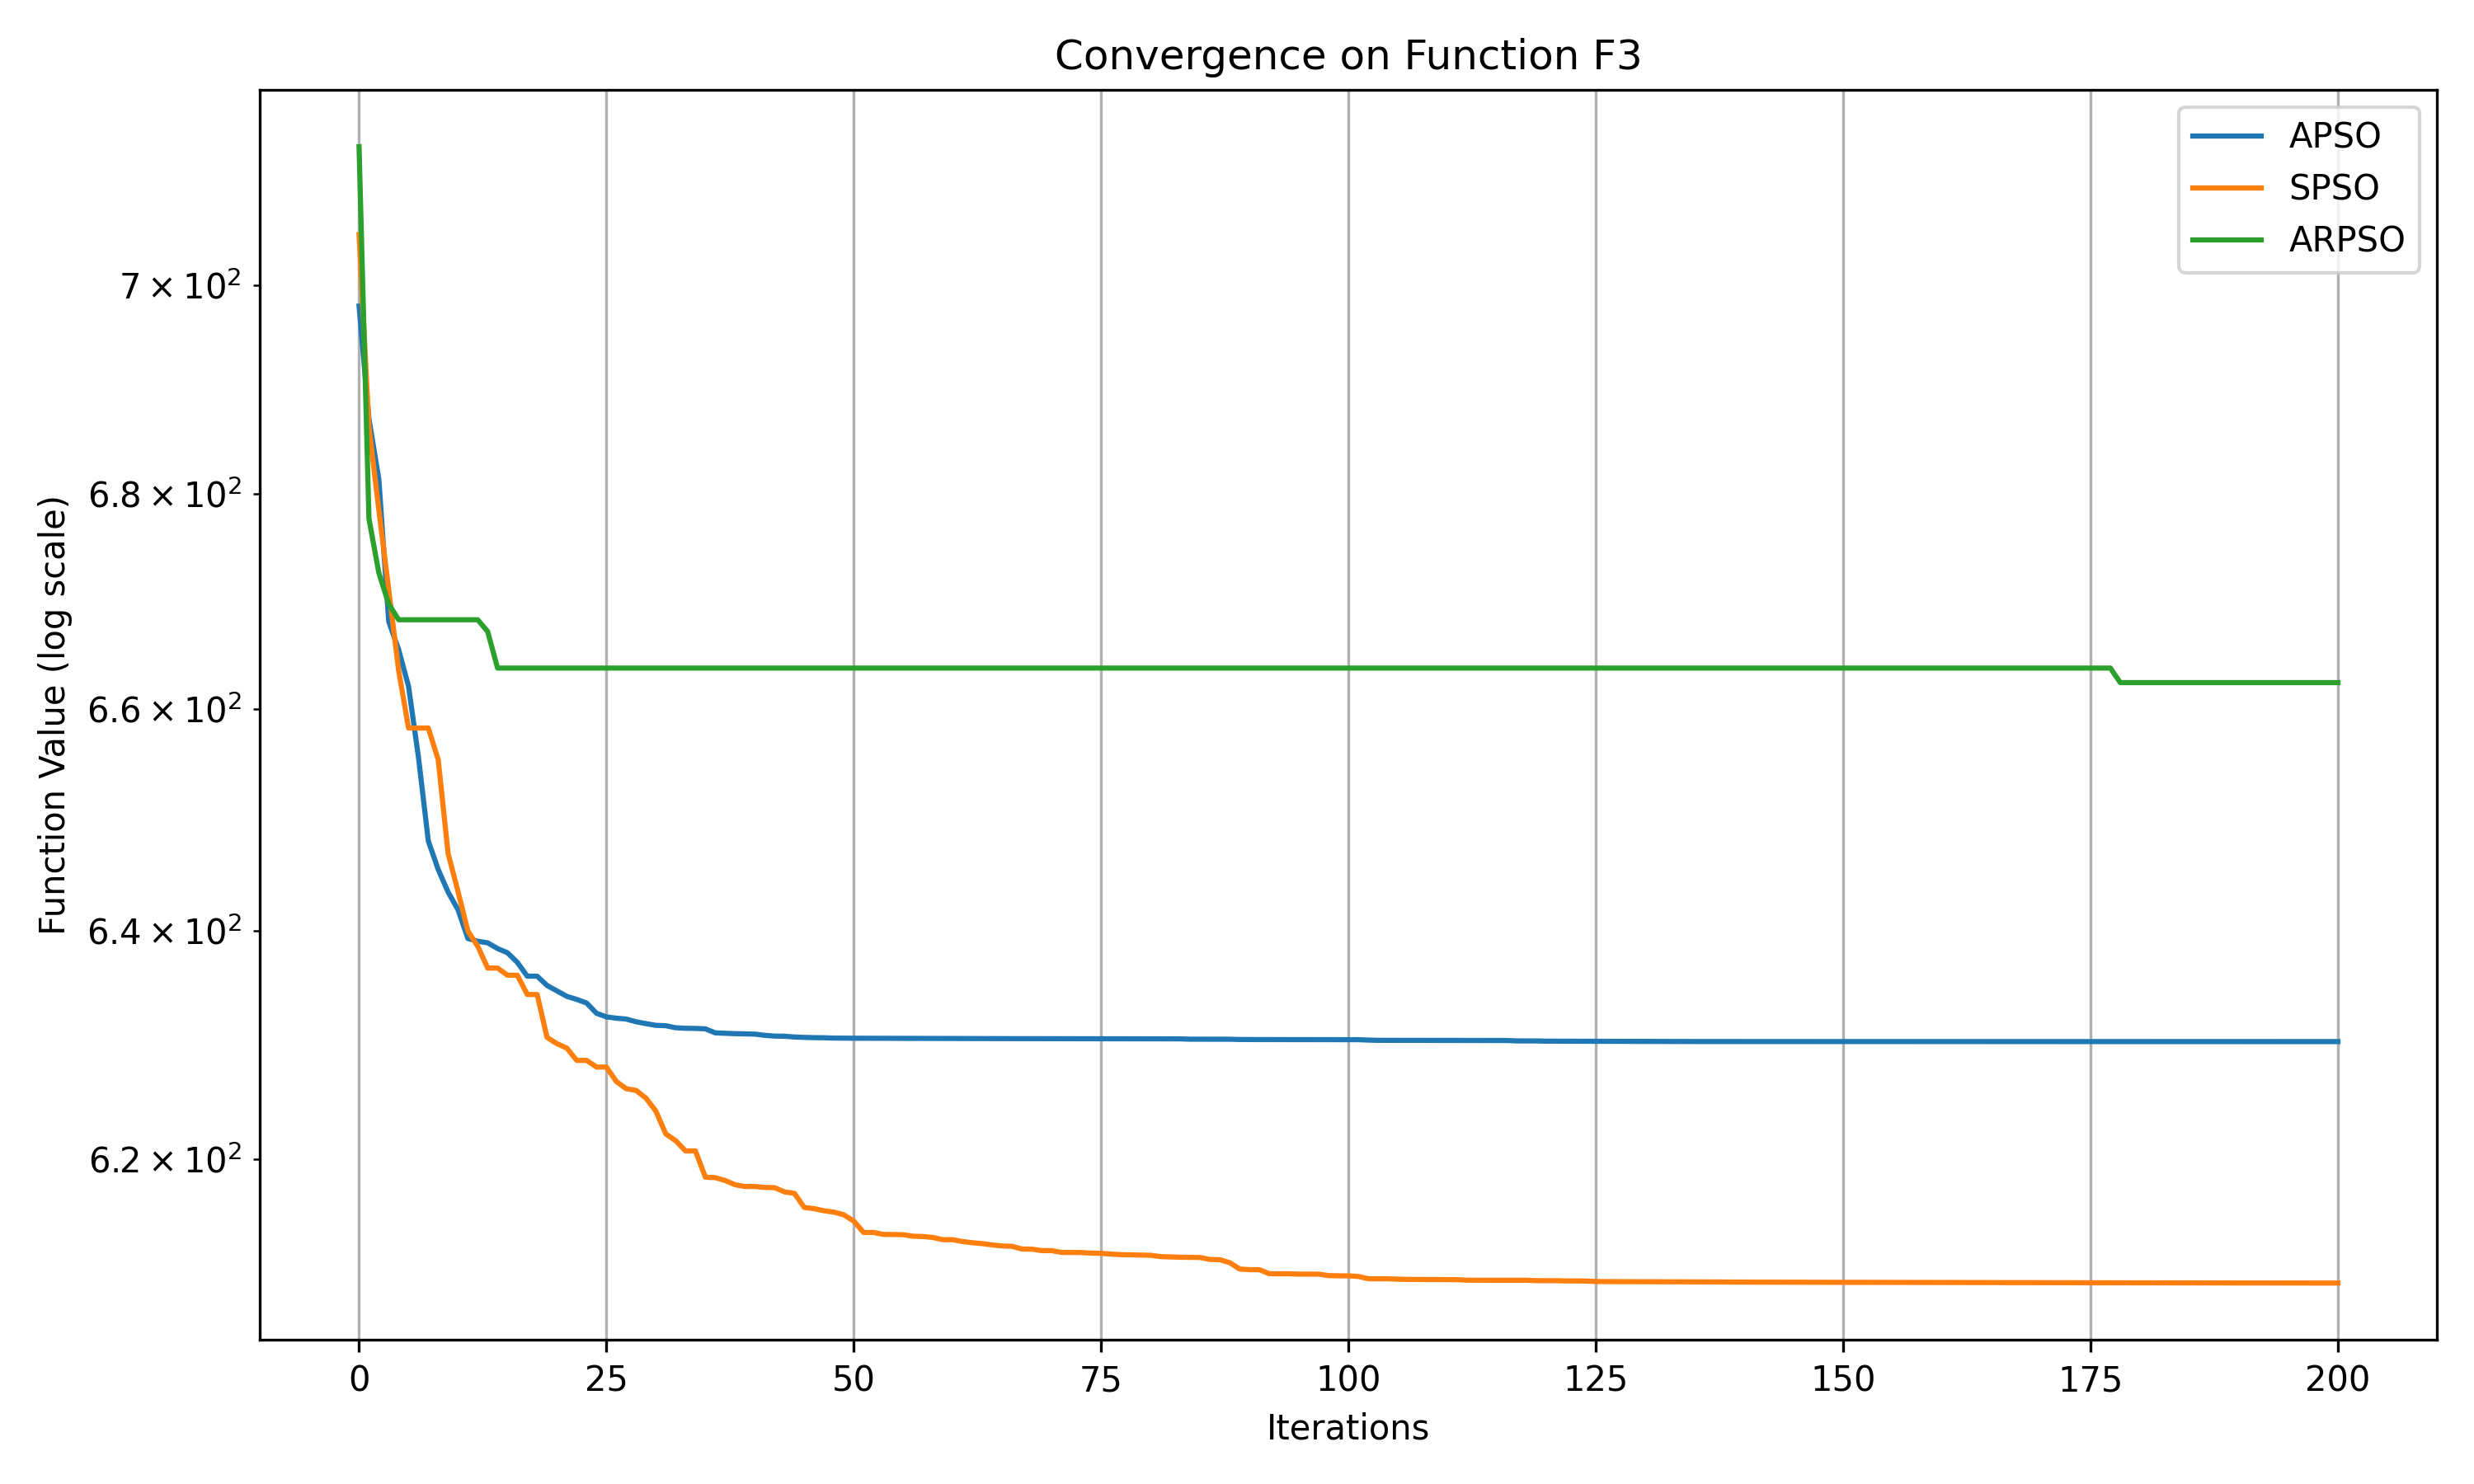
\includegraphics[width=\linewidth]{../plots/cec_bench/cec_convergence_f3.png}
    \caption{F3 (Schaffer)}
    \label{fig:conv_f3}
\end{subfigure}

\vspace{0.5cm}
\begin{subfigure}{0.32\linewidth}
    \centering
    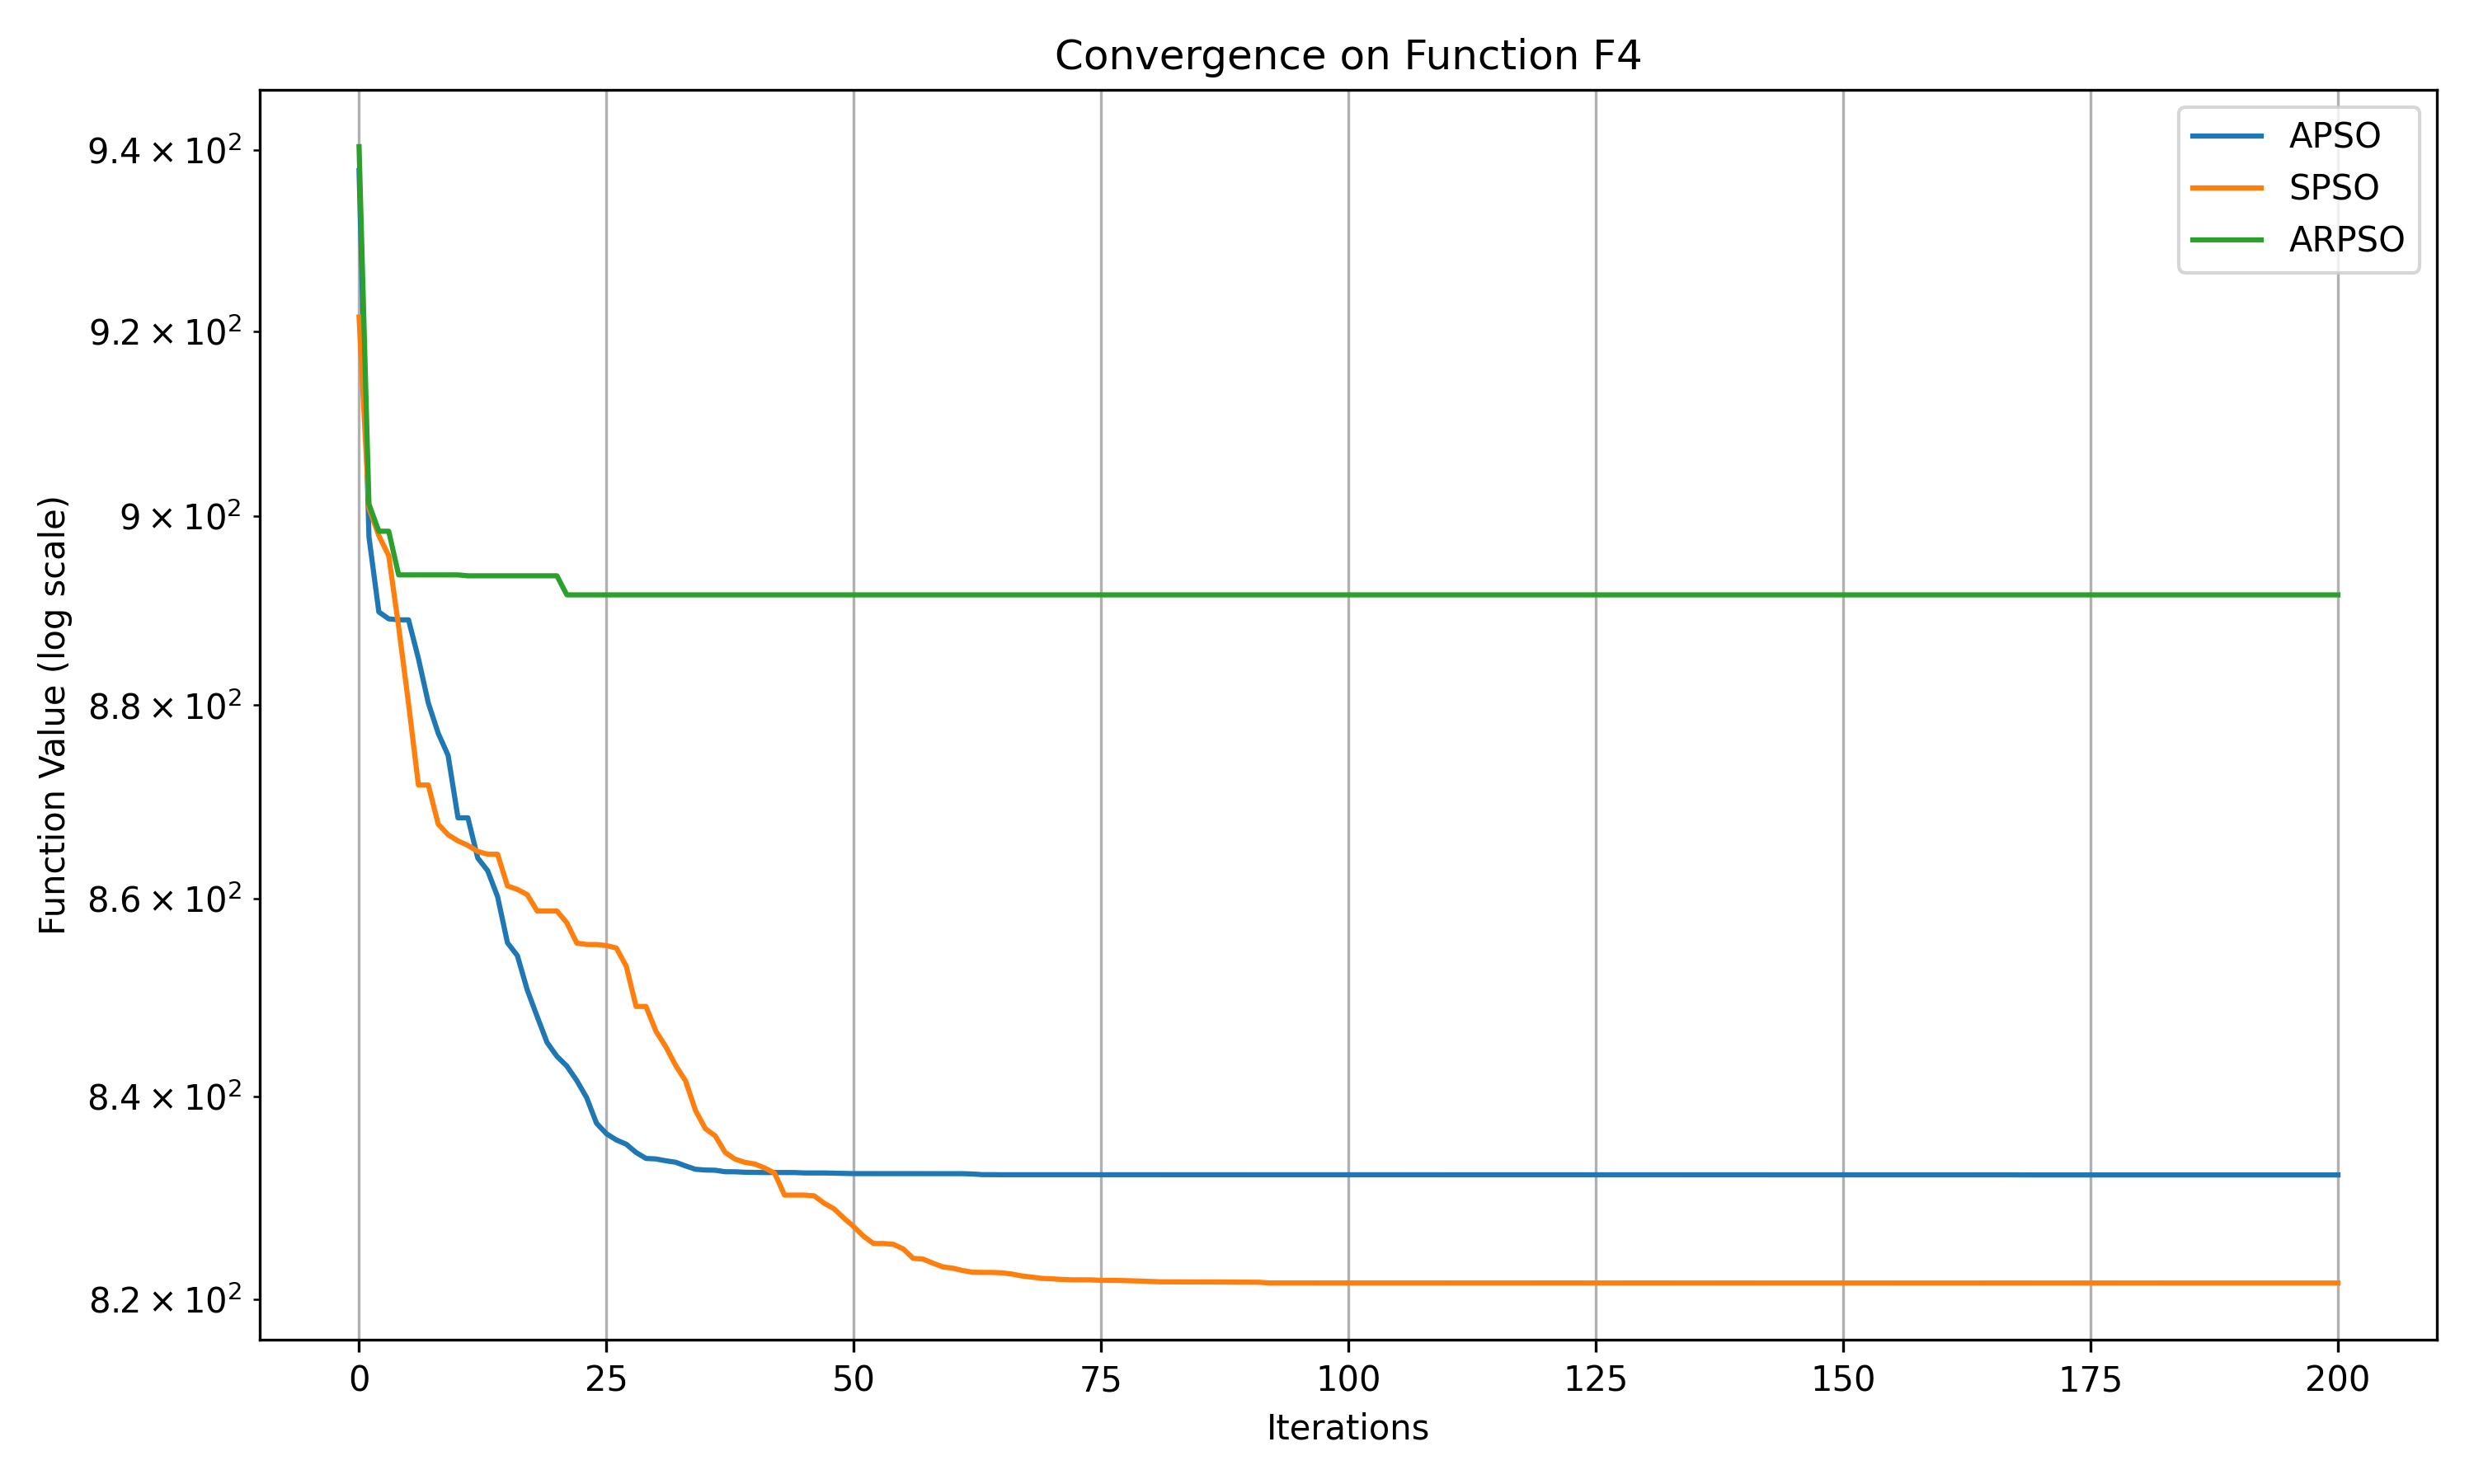
\includegraphics[width=\linewidth]{../plots/cec_bench/cec_convergence_f4.png}
    \caption{F4 (Step Rastrigin)}
    \label{fig:conv_f4}
\end{subfigure}
\hfill
\begin{subfigure}{0.32\linewidth}
    \centering
    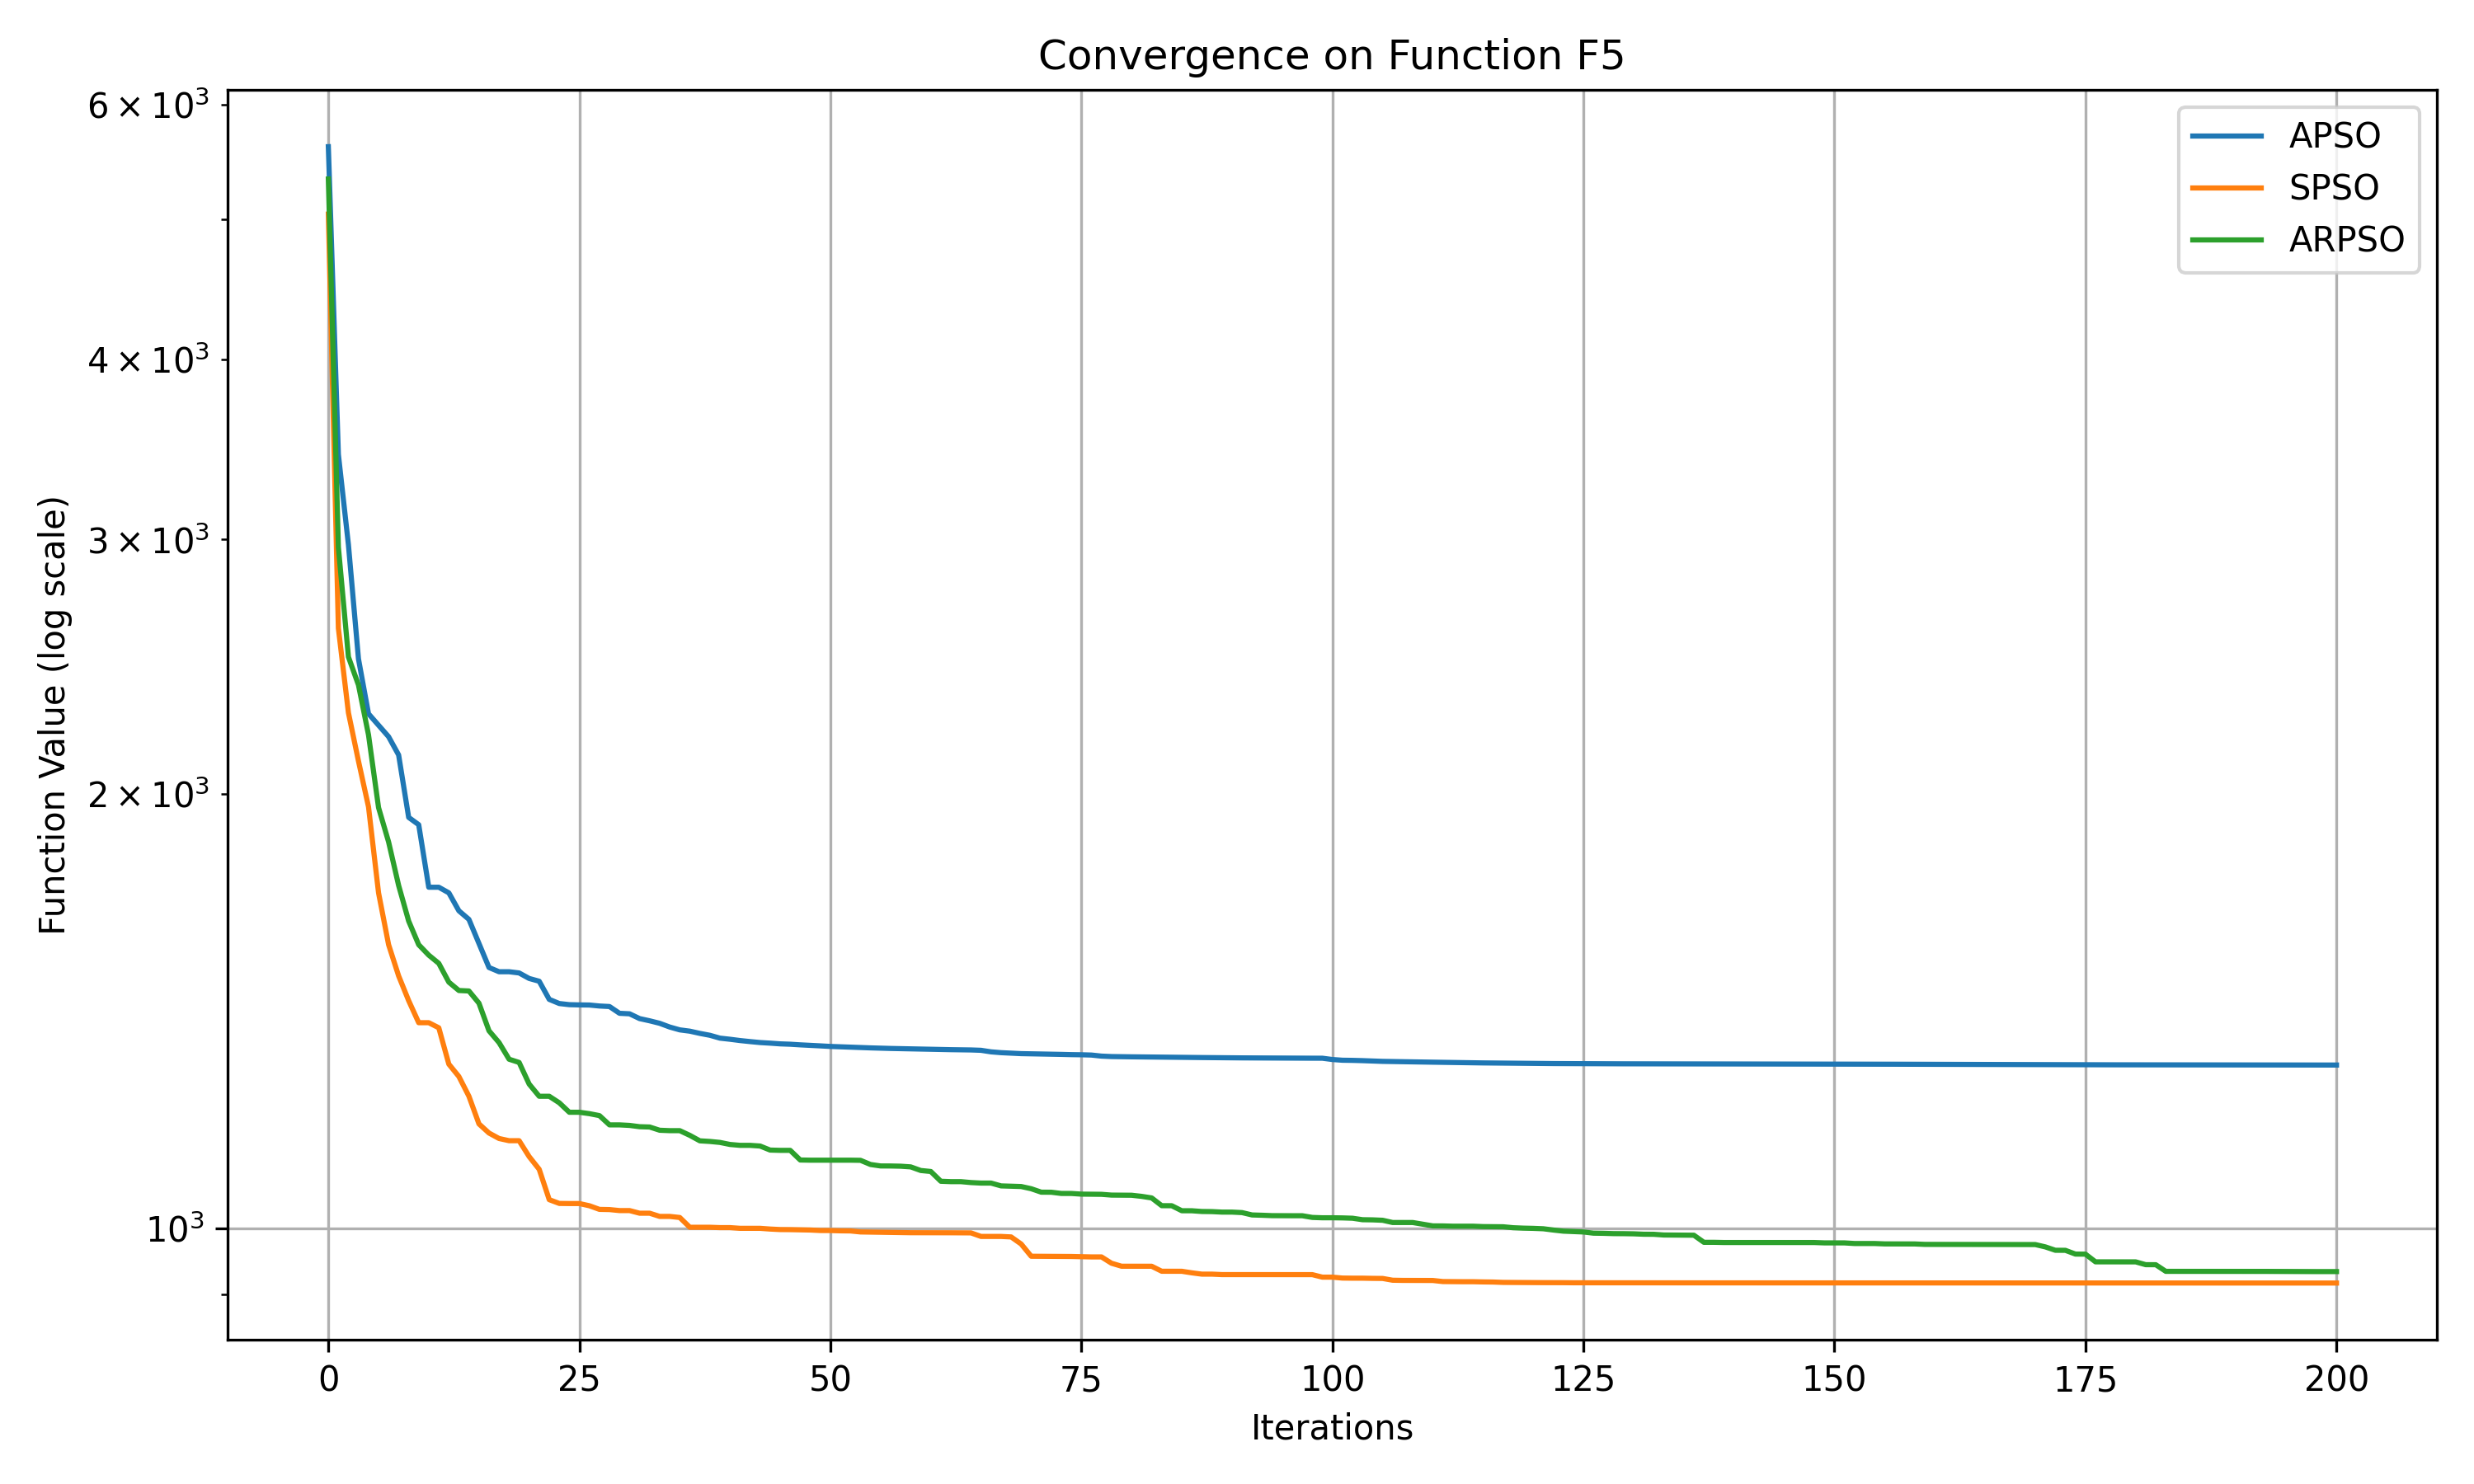
\includegraphics[width=\linewidth]{../plots/cec_bench/cec_convergence_f5.png}
    \caption{F5 (Levy)}
    \label{fig:conv_f5}
\end{subfigure}

\caption{Convergence plots for PSO variants on CEC 2022 benchmark functions}
\label{fig:convergence_plots}
\end{figure}

Table \ref{tab:benchmark_results} summarizes the mean and standard deviation of the final function values achieved by each algorithm across the five benchmark functions.

\begin{table}[htbp]
\caption{Mean Function Values Across Benchmark Functions}
\begin{center}
\begin{tabular}{|c|c|c|c|c|c|}
\hline
\textbf{Algorithm} & \textbf{F1} & \textbf{F2} & \textbf{F3} & \textbf{F4} & \textbf{F5} \\
\hline
APSO & 2.14e+03 & 4.45e+02 & 6.30e+02 & 8.32e+02 & 1.30e+03 \\
\hline
SPSO & 6.86e+02 & 4.55e+02 & 6.09e+02 & 8.22e+02 & 9.17e+02 \\
\hline
ARPSO & 1.49e+03 & \textbf{4.17e+02} & 6.62e+02 & 8.92e+02 & 9.34e+02 \\
\hline
\end{tabular}
\label{tab:benchmark_results}
\end{center}
\end{table}

Fig. 4 shows a radar chart comparing the relative performance of the three PSO variants across the five benchmark functions.

\begin{figure}[htbp]
\centering
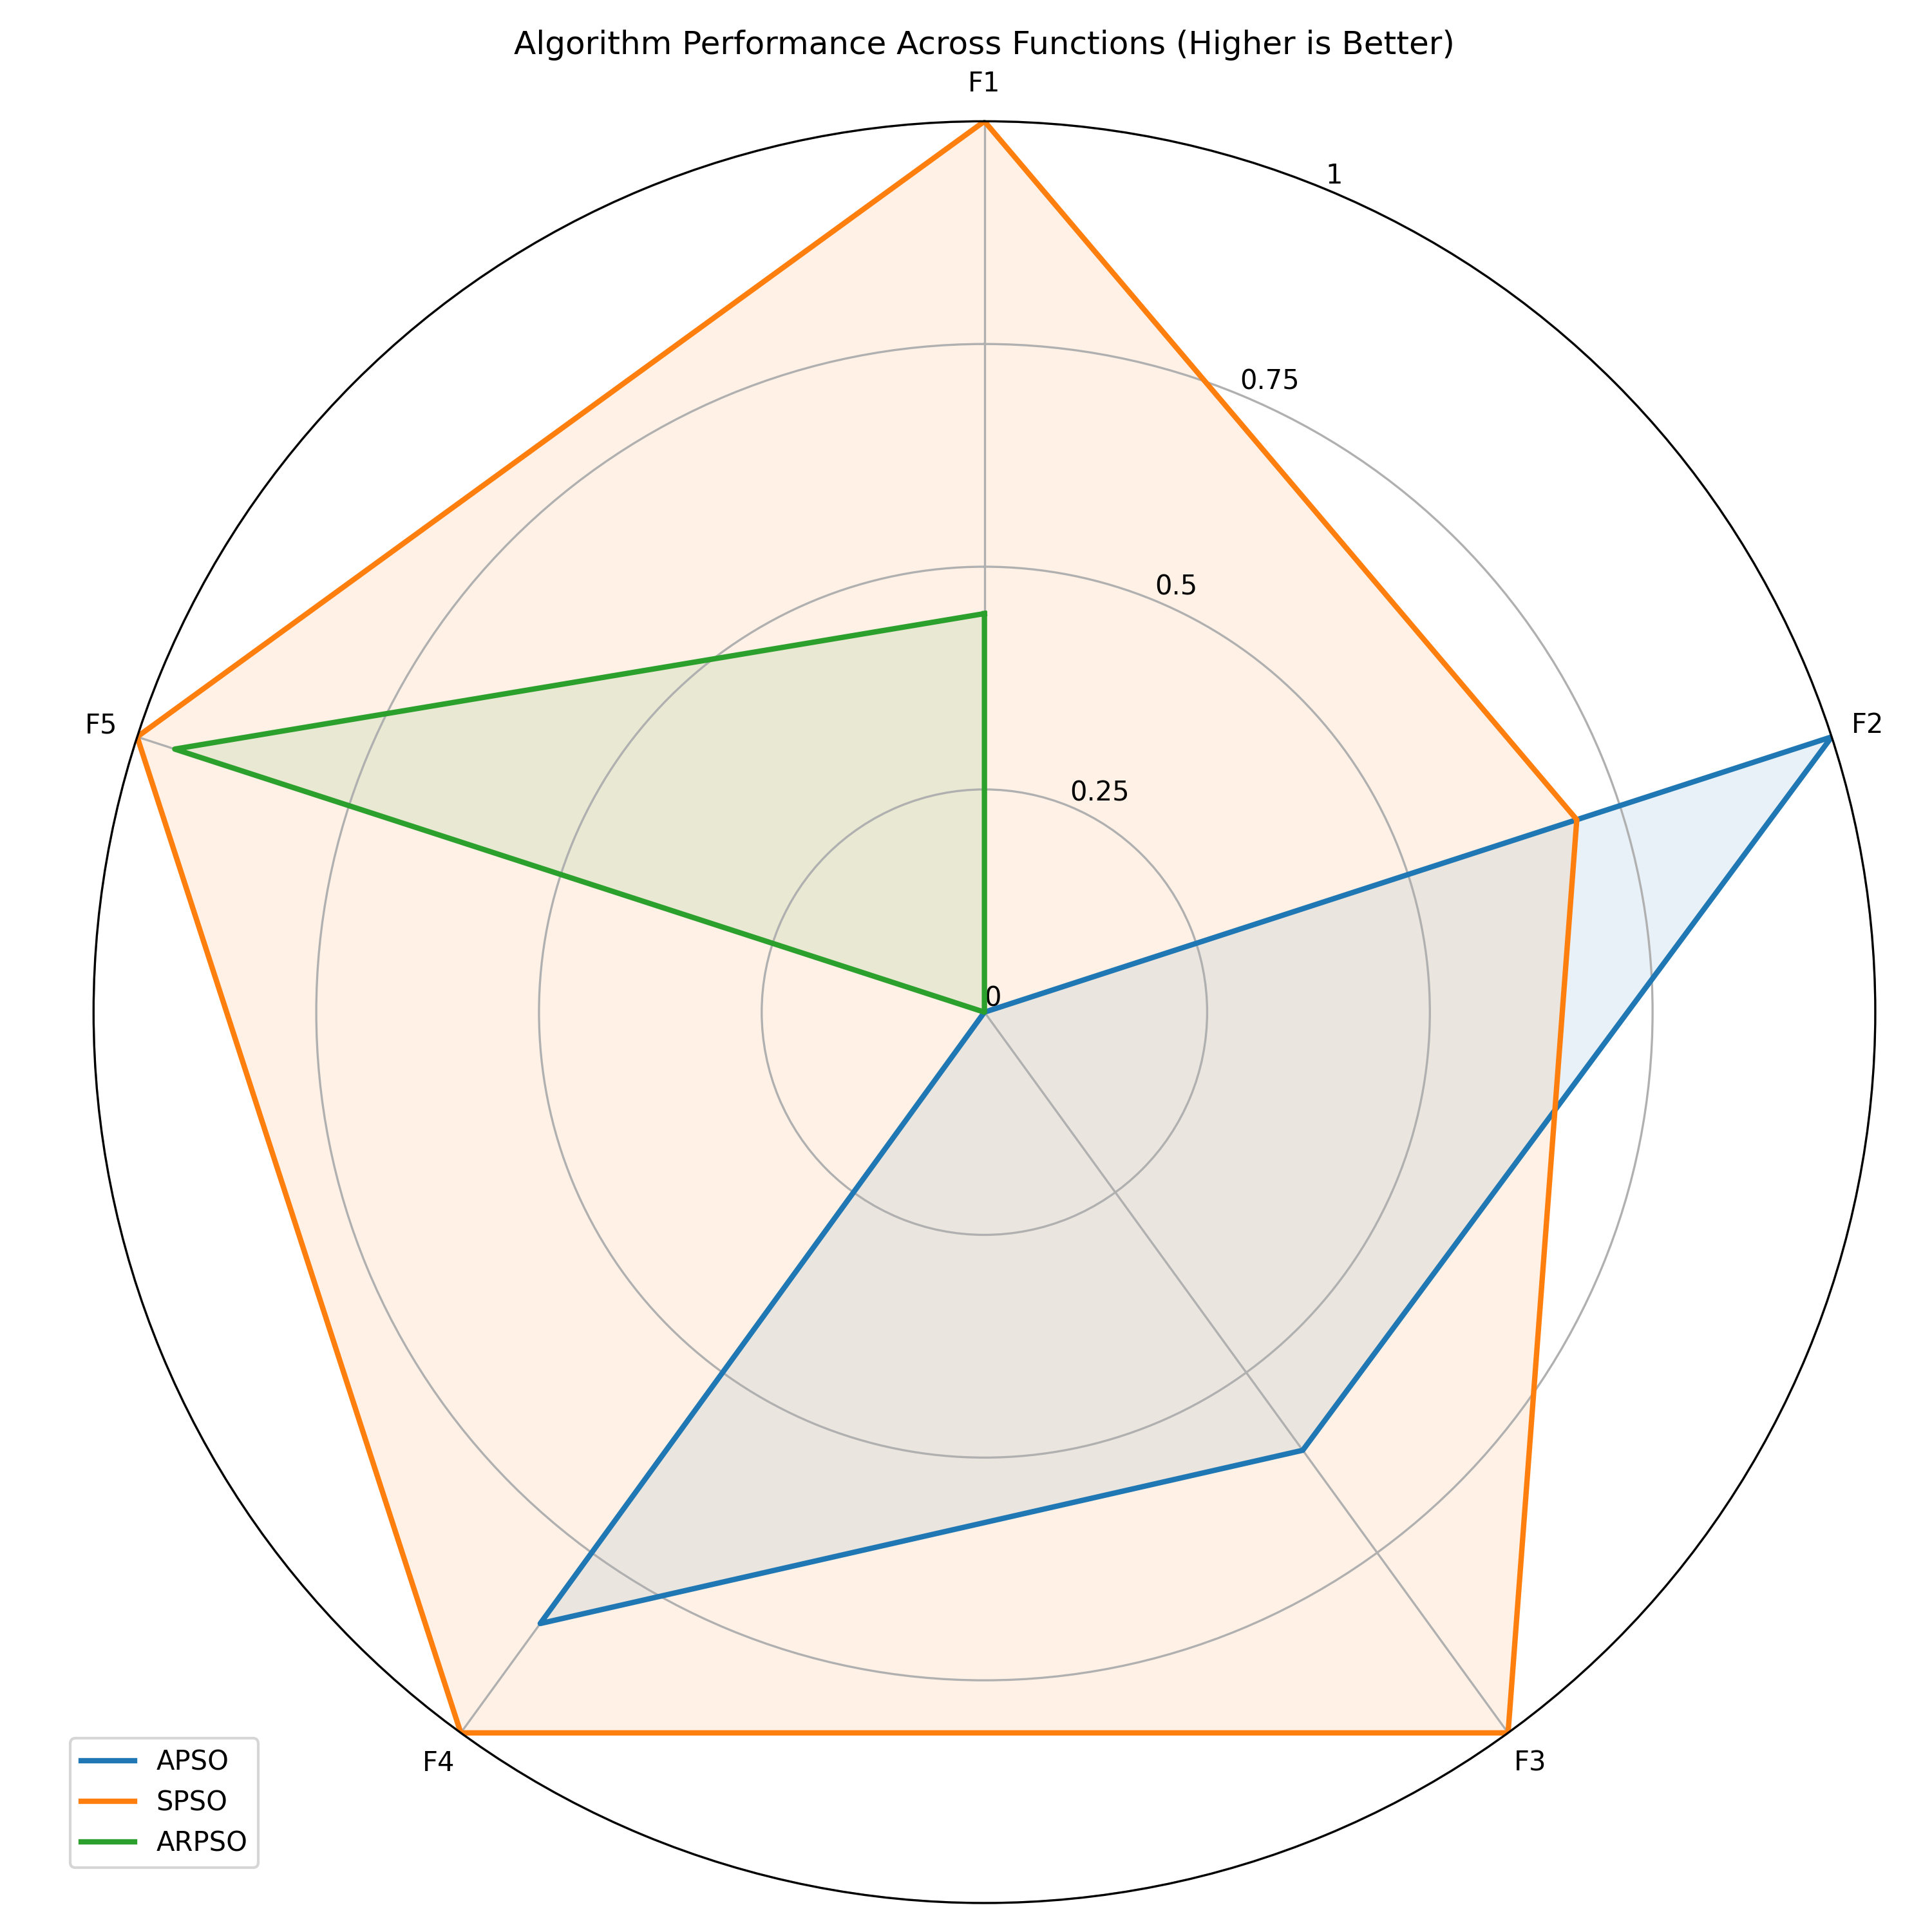
\includegraphics[width=0.7\linewidth]{../plots/cec_bench/radar_chart.png}
\caption{Radar chart of PSO performance across benchmark functions}
\label{fig:radar_chart}
\end{figure}

\subsection{Discussion}
The benchmark results reveal a different performance pattern compared to the source seeking experiments:

\begin{itemize}
    \item SPSO performs best overall, winning on 4 out of 5 functions (F1, F3, F4, F5)
    \item ARPSO shows mixed performance, winning on F2 (Rosenbrock) but struggling with other functions
    \item APSO consistently underperforms on most benchmark functions compared to SPSO, though it shows competitive performance on F2
\end{itemize}

These results can be explained by the characteristics of the algorithms and the nature of the benchmark functions:

\begin{itemize}
    \item SPSO's balanced exploration-exploitation approach works well for diverse optimization challenges
    \item APSO's momentum can be advantageous for functions with narrow valleys (like Rosenbrock) but may cause overshooting in other cases
    \item ARPSO's focus on exploration through randomness can make precise convergence difficult
\end{itemize}

The convergence plots provide additional insights:

\begin{itemize}
    \item APSO shows faster initial convergence on some functions (F2, F4) but plateaus earlier
    \item SPSO demonstrates steady, consistent improvement and achieves the best final solutions on most functions
    \item ARPSO plateaus early on several functions but occasionally shows late improvements
\end{itemize}

These observations suggest that each PSO variant has complementary strengths that could potentially be combined in hybrid approaches.

\section{Hybrid PSO Approaches}
\subsection{Hybrid Strategies}
Based on the complementary strengths observed in the PSO variants, we developed four hybrid approaches:

\subsubsection{Particle Hybrid}
In this approach, different particles within the same swarm use different update rules:
\begin{itemize}
    \item The swarm is divided into 3 groups of 10 particles each
    \item Group 1: APSO update rules
    \item Group 2: SPSO update rules
    \item Group 3: ARPSO update rules
    \item All particles share information about the global best position
\end{itemize}

\subsubsection{Sequential Hybrid}
This approach uses different algorithms in sequence:
\begin{itemize}
    \item Phase 1: APSO runs for 40\% of total iterations
    \item Phase 2: SPSO is initialized around APSO's final solution and runs for 60\% of iterations
    \item The best solution from APSO is used as a starting point for SPSO
\end{itemize}

\subsubsection{Parallel Hybrid}
In this approach, multiple algorithms run simultaneously on separate sub-swarms:
\begin{itemize}
    \item Three separate swarms run in parallel (10 particles each)
    \item Swarm 1: APSO
    \item Swarm 2: SPSO
    \item Swarm 3: ARPSO
    \item After each iteration, the best solution across all swarms is shared with all algorithms
\end{itemize}

\subsubsection{Adaptive Hybrid}
This approach dynamically switches between algorithms based on their recent performance:
\begin{itemize}
    \item Maintains three algorithm instances (APSO, SPSO, ARPSO)
    \item Starts with APSO
    \item Every 10 iterations, evaluates which algorithm has made the most improvement
    \item Switches to the best-performing algorithm for the next 10 iterations
    \item All algorithms share the same global best information
\end{itemize}

\subsection{Experimental Setup}
We evaluated the hybrid approaches on the same five CEC 2022 benchmark functions used in Section IV. The experimental parameters were:
\begin{itemize}
    \item Dimension: 10
    \item Total number of particles: 30 (distributed as described for each hybrid approach)
    \item Maximum iterations: 200
    \item Number of runs: 5 for each function and algorithm
\end{itemize}

\subsection{Results}
Fig. 5 shows the convergence behavior of the hybrid approaches compared to the original PSO variants on the five benchmark functions.

\begin{figure}[htbp]
\centering
\begin{subfigure}{0.32\linewidth}
    \centering
    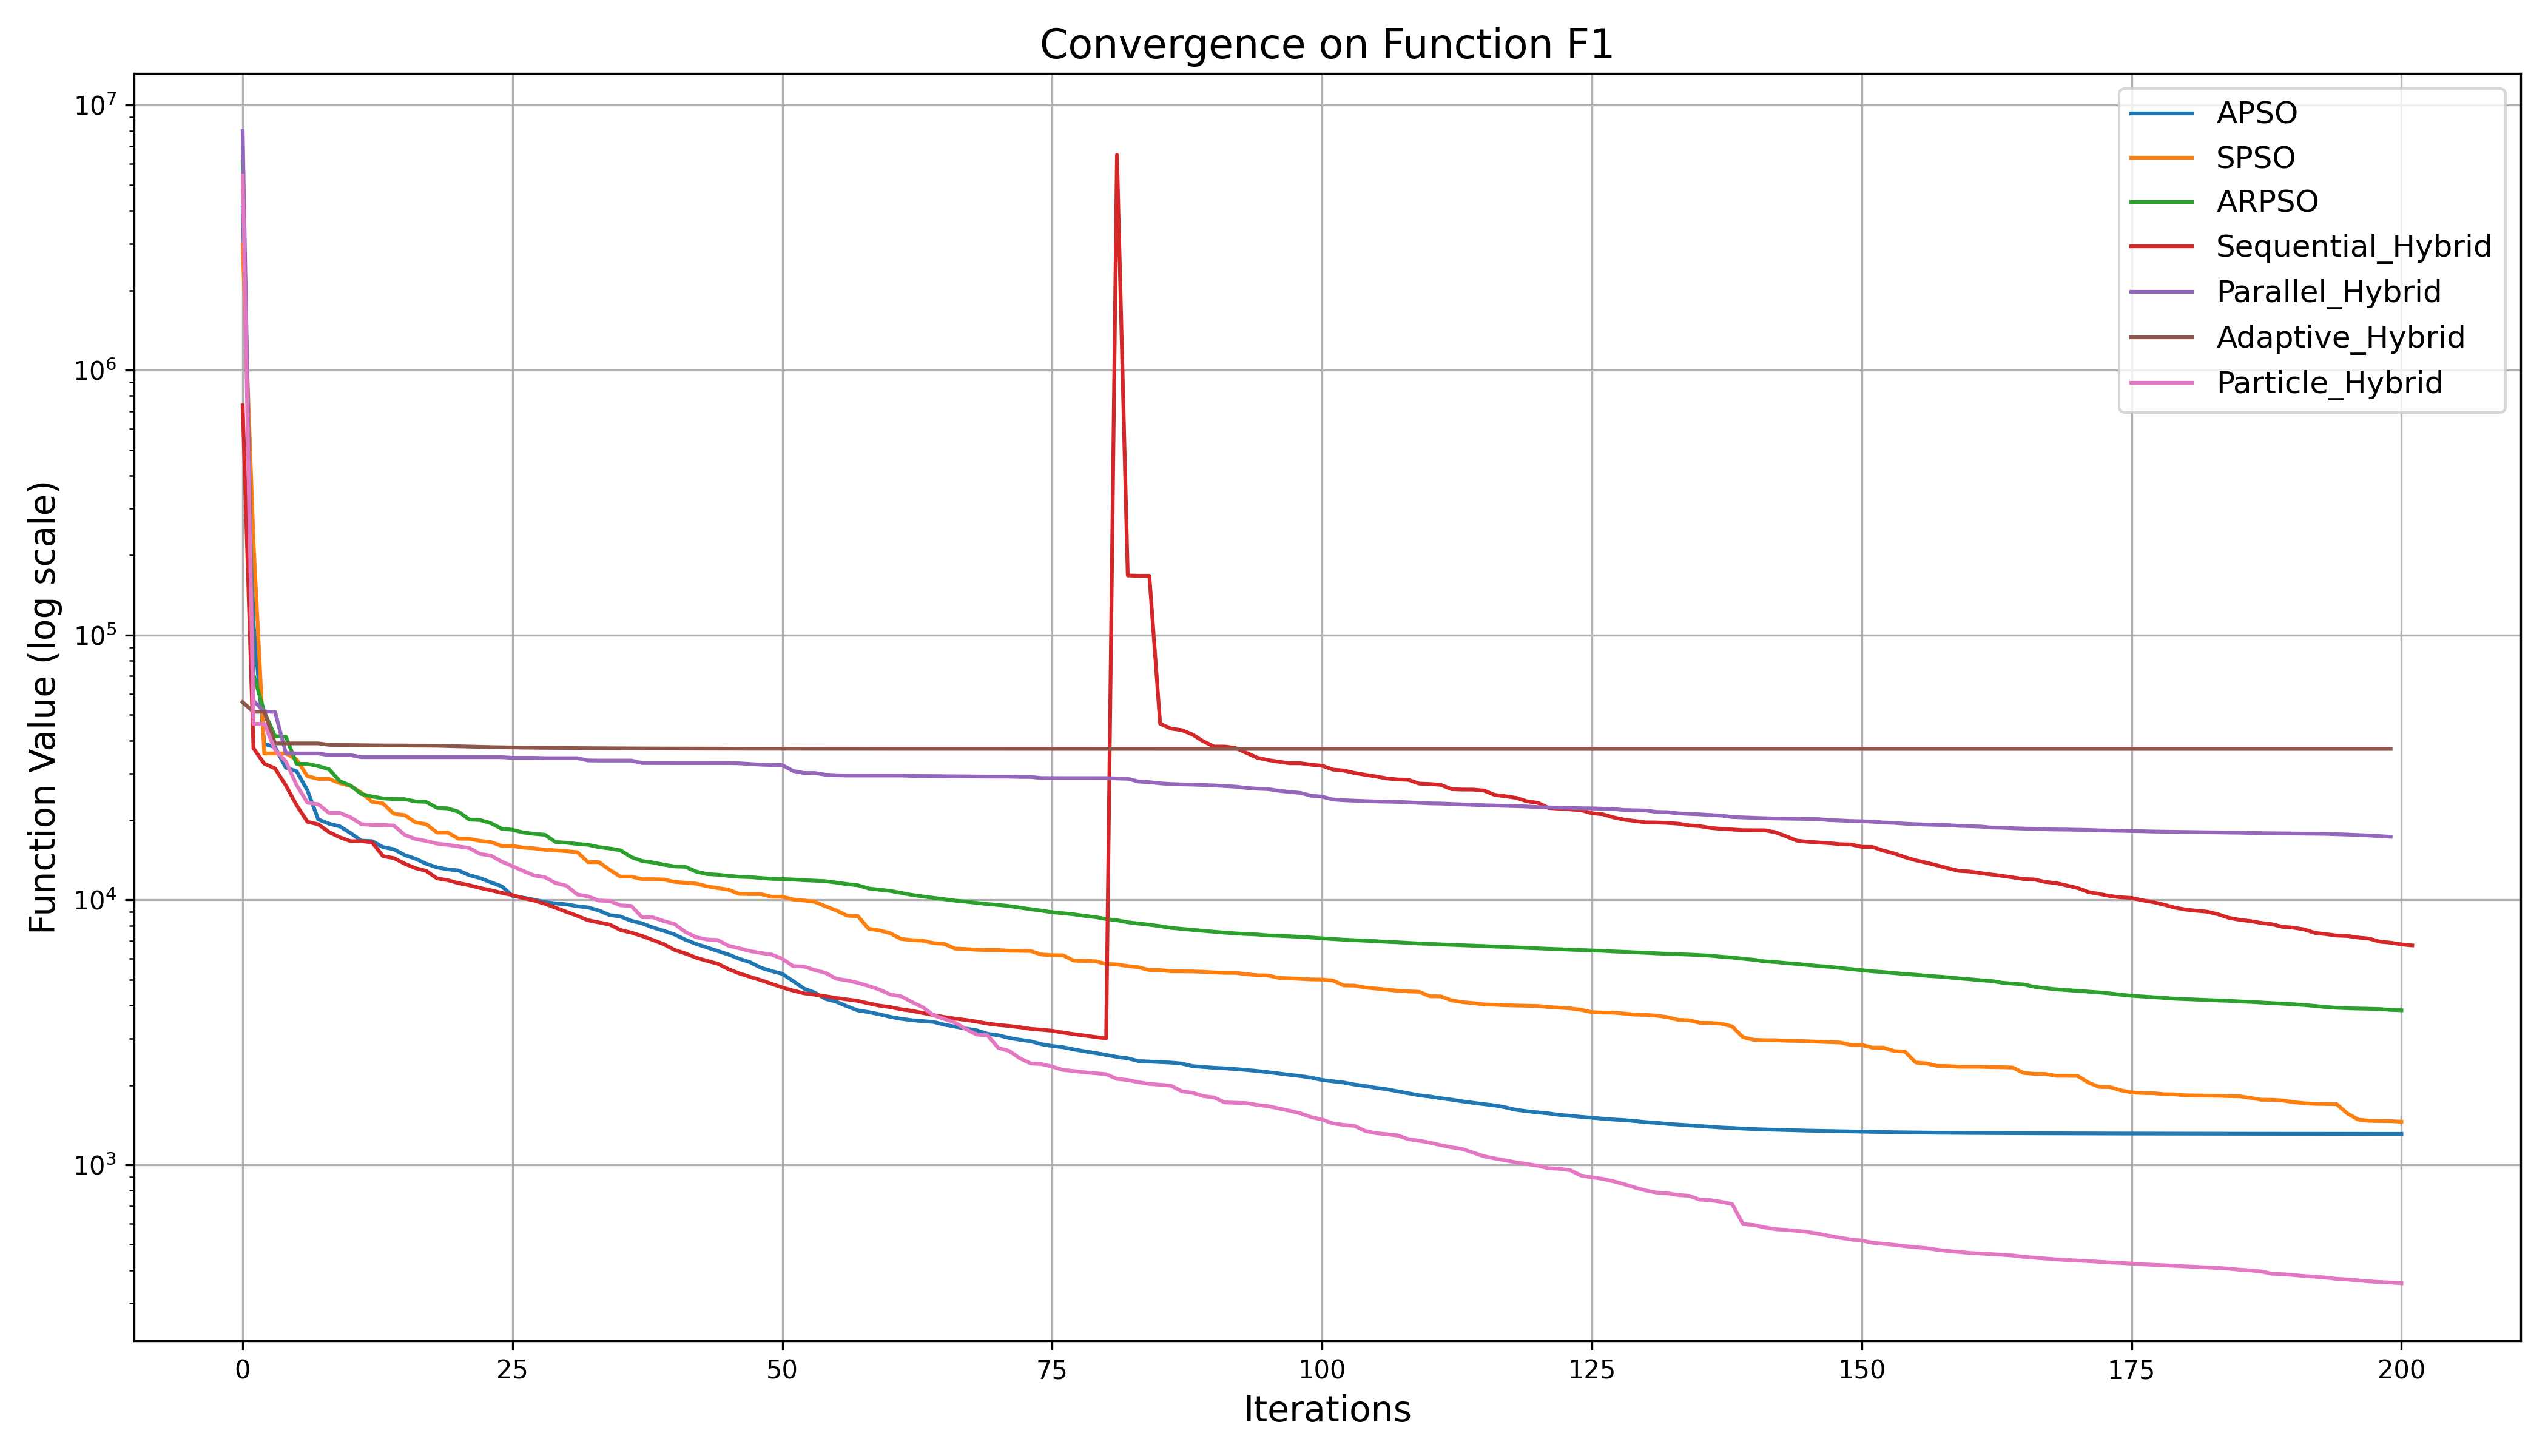
\includegraphics[width=\linewidth]{../plots/exploitation/hybrid_convergence_f1.png}
    \caption{F1 (Zakharov)}
    \label{fig:hybrid_conv_f1}
\end{subfigure}
\hfill
\begin{subfigure}{0.32\linewidth}
    \centering
    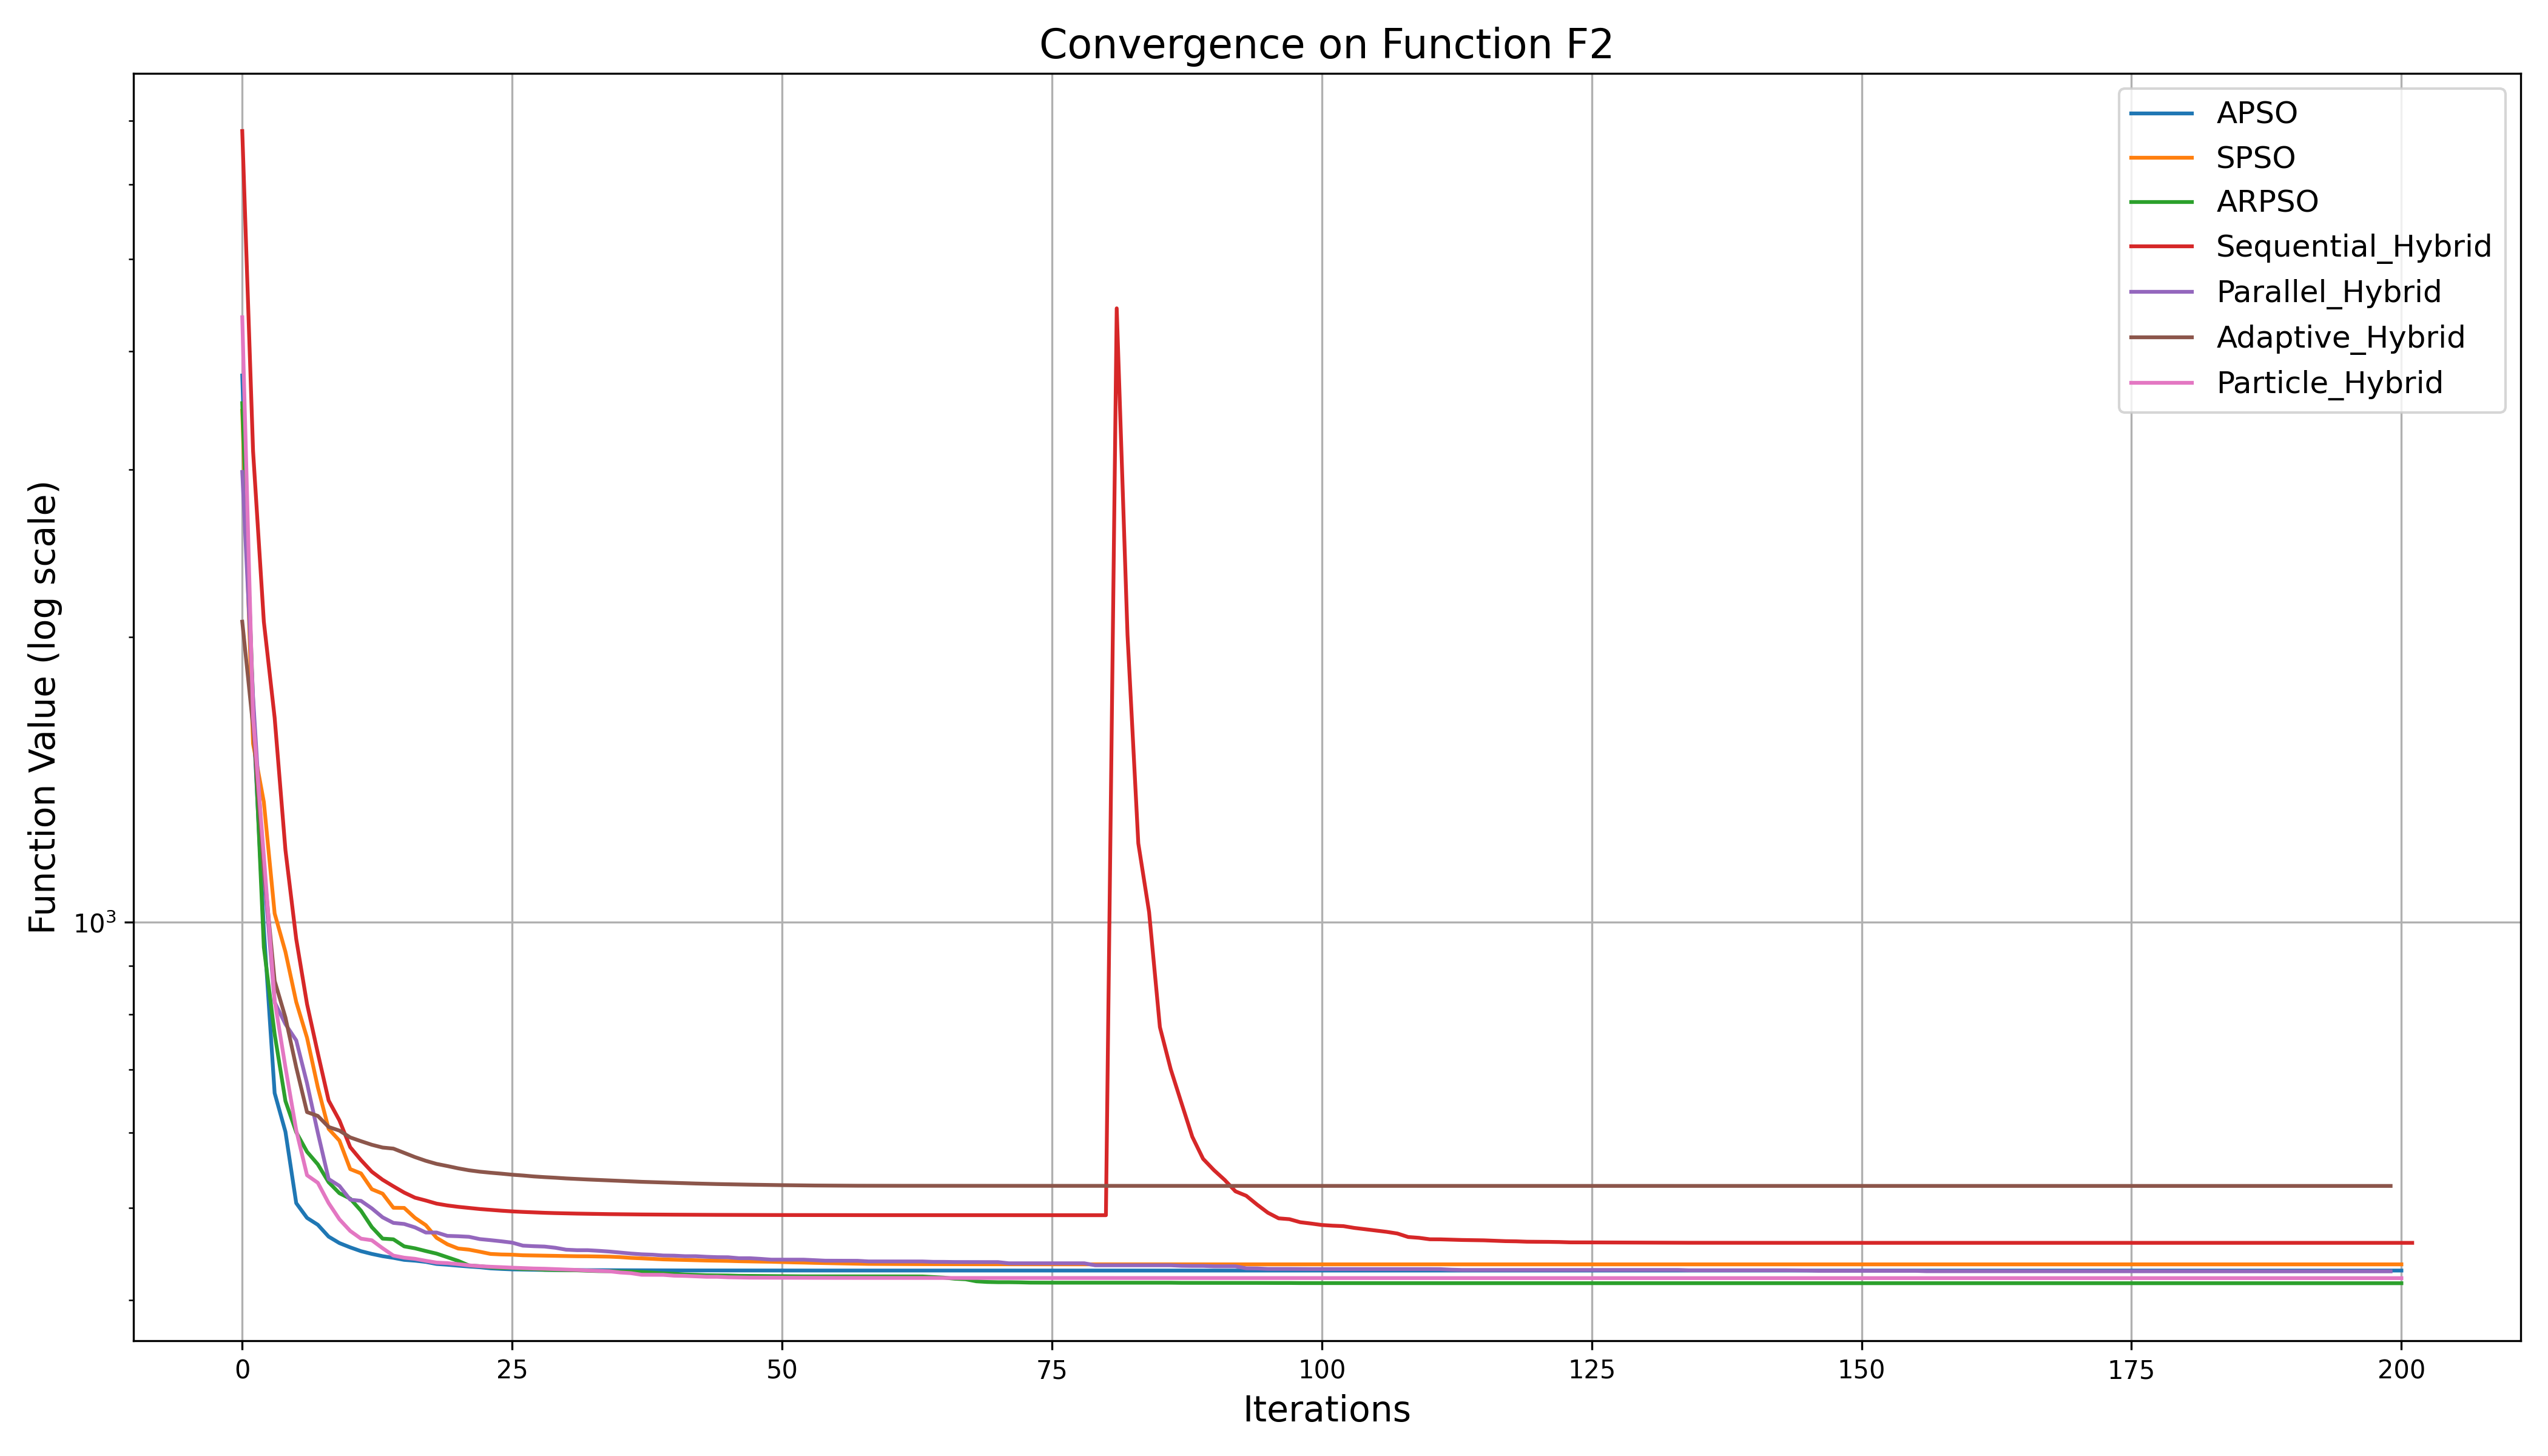
\includegraphics[width=\linewidth]{../plots/exploitation/hybrid_convergence_f2.png}
    \caption{F2 (Rosenbrock)}
    \label{fig:hybrid_conv_f2}
\end{subfigure}
\hfill
\begin{subfigure}{0.32\linewidth}
    \centering
    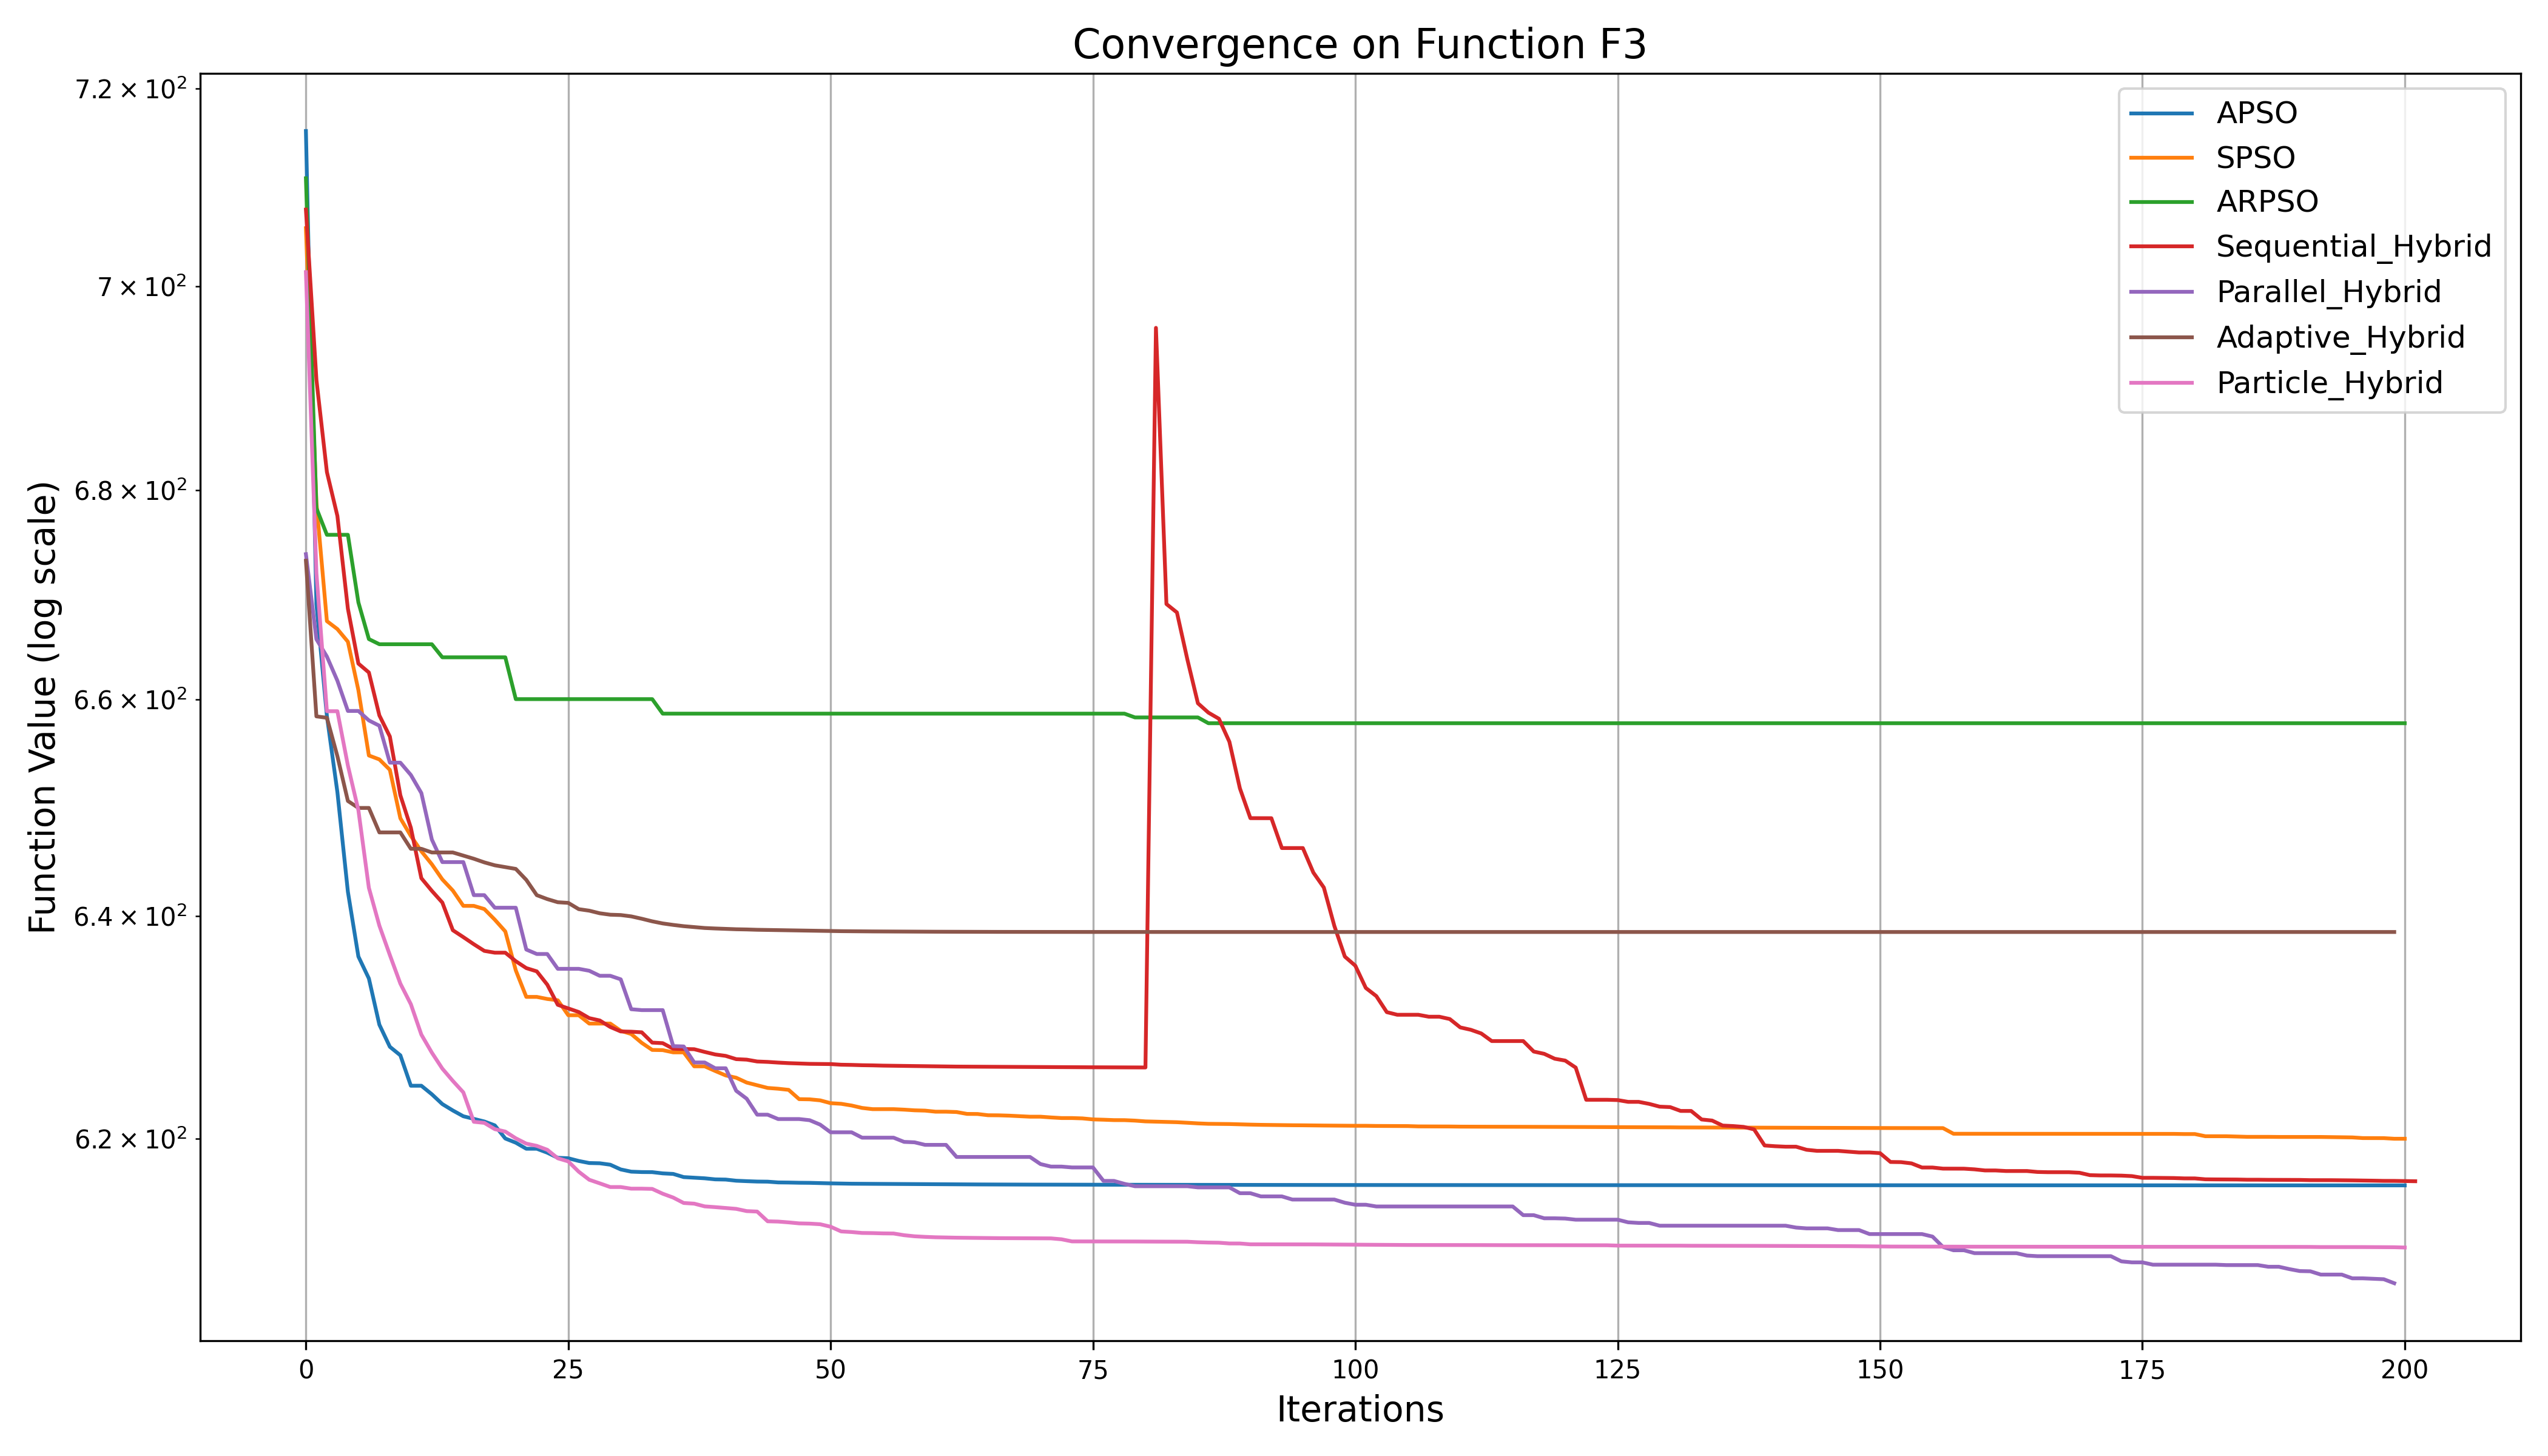
\includegraphics[width=\linewidth]{../plots/exploitation/hybrid_convergence_f3.png}
    \caption{F3 (Schaffer)}
    \label{fig:hybrid_conv_f3}
\end{subfigure}

\vspace{0.5cm}
\begin{subfigure}{0.32\linewidth}
    \centering
    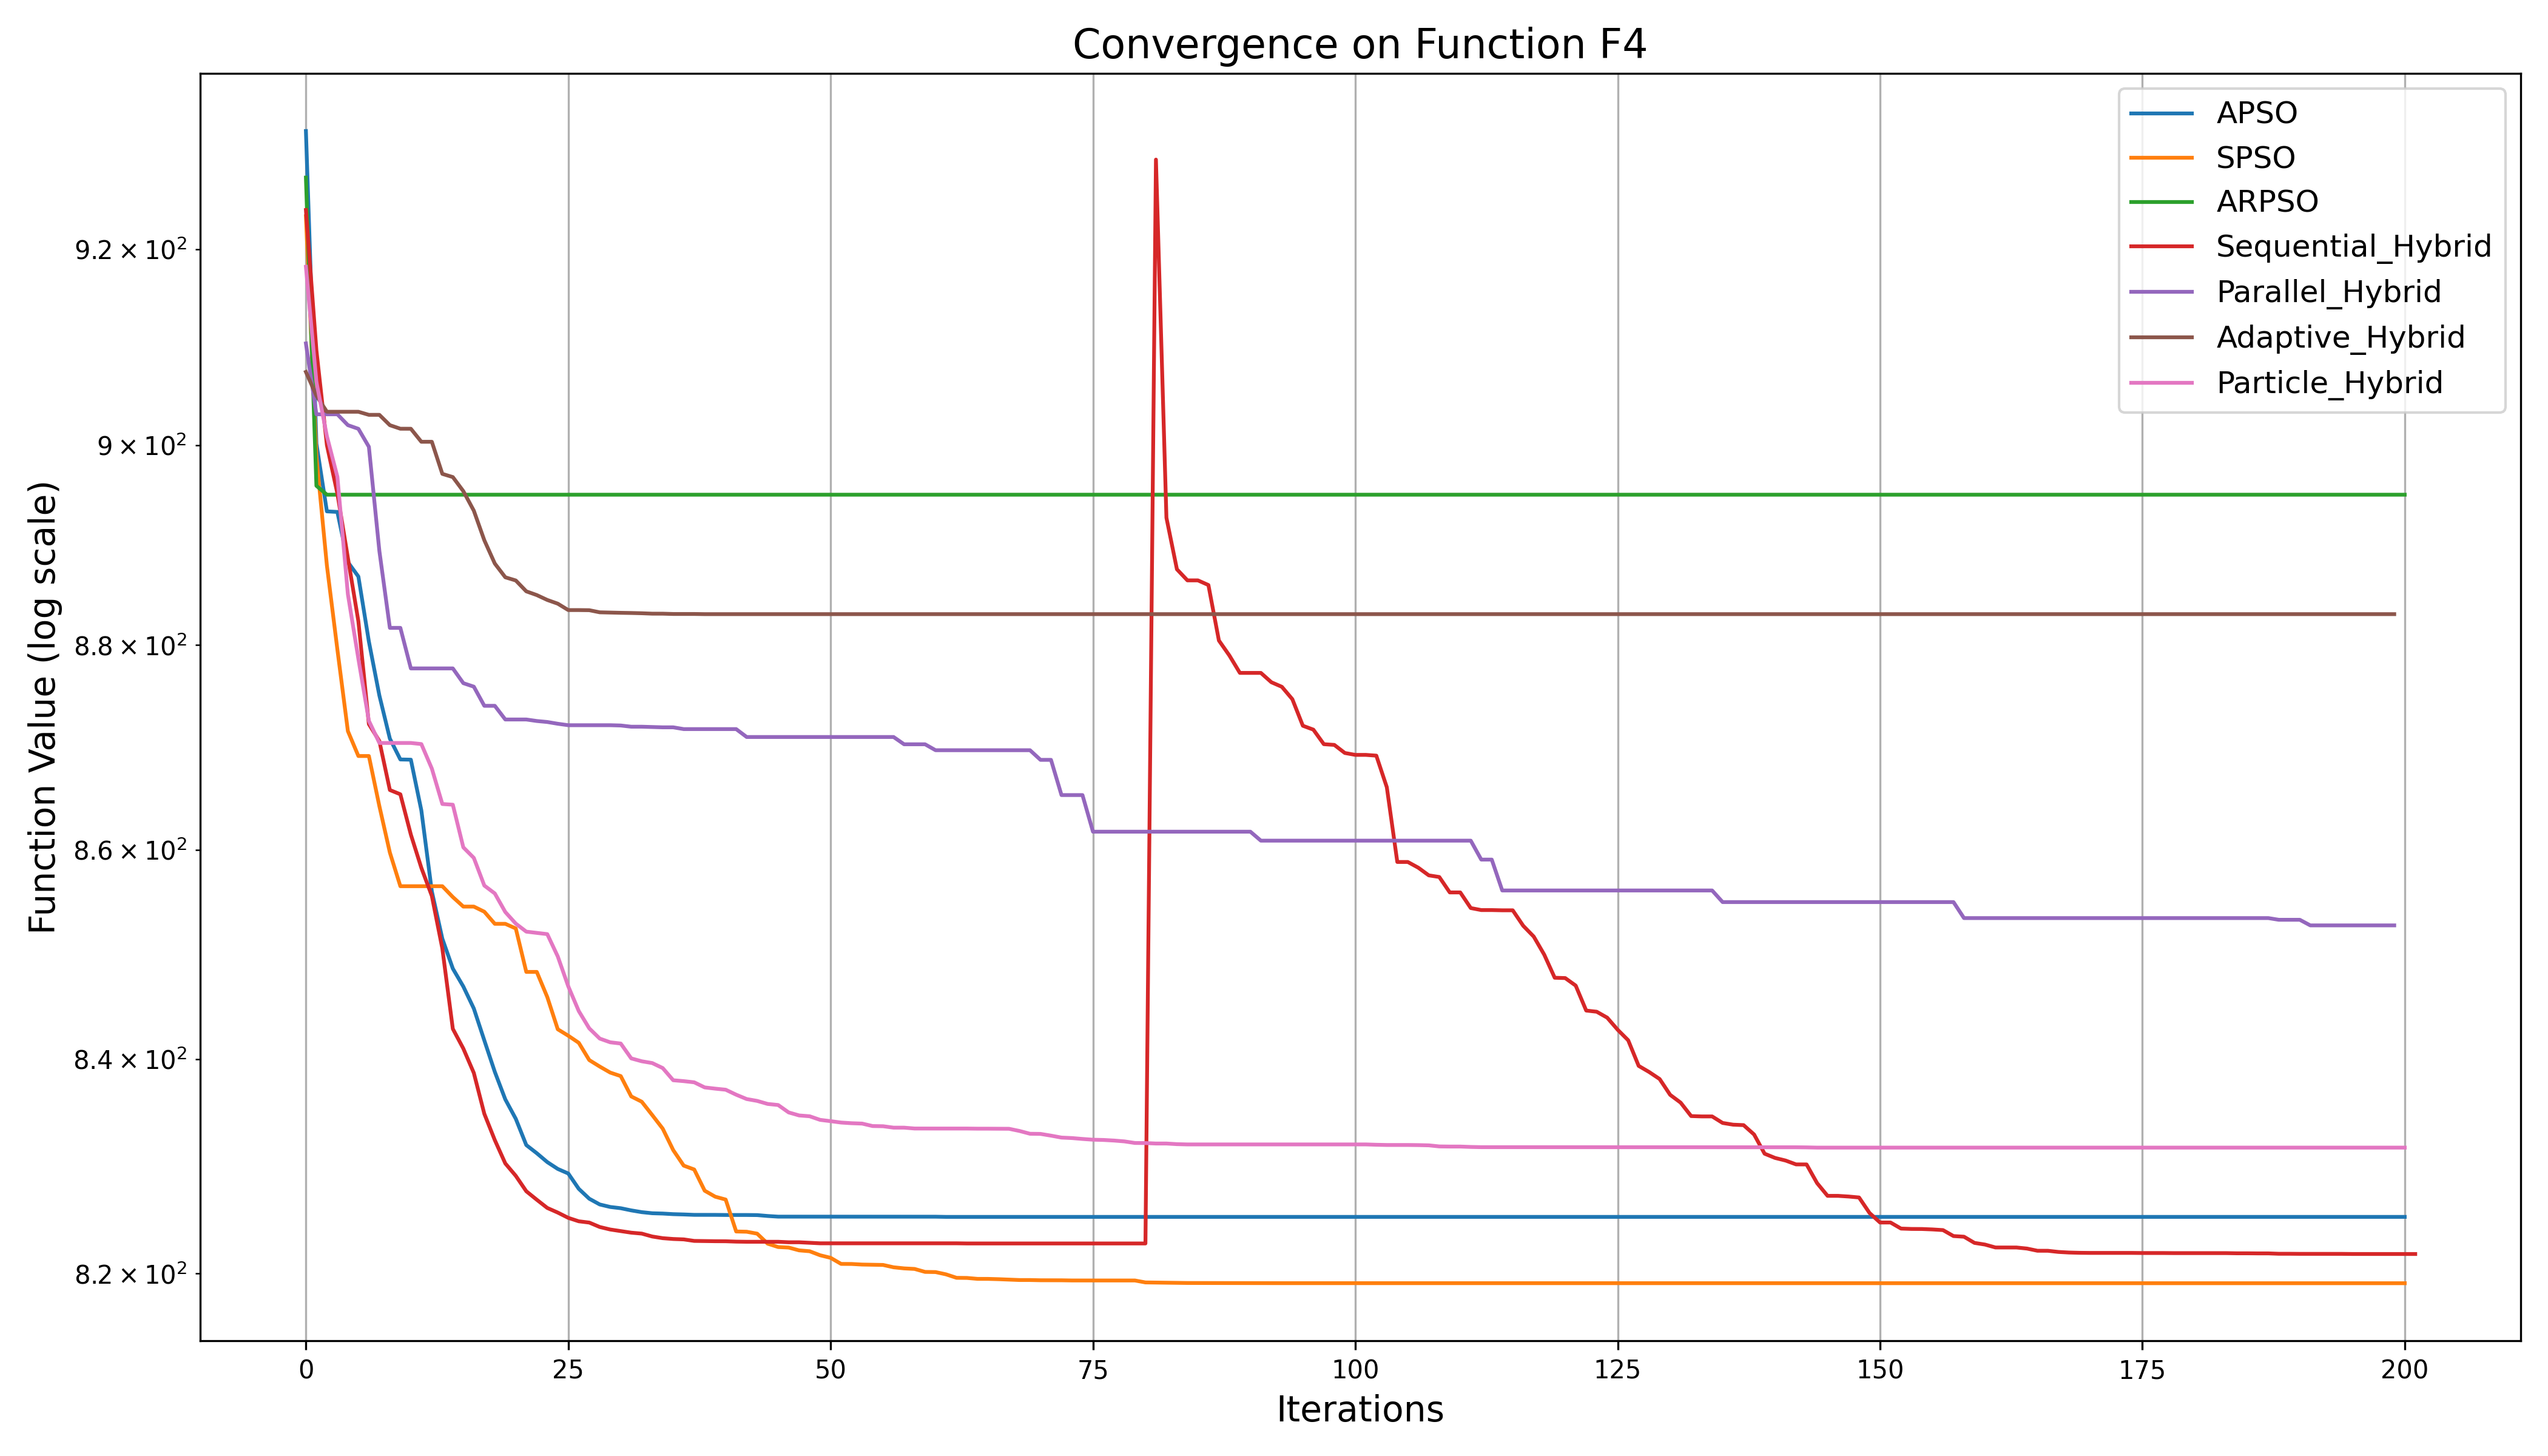
\includegraphics[width=\linewidth]{../plots/exploitation/hybrid_convergence_f4.png}
    \caption{F4 (Step Rastrigin)}
    \label{fig:hybrid_conv_f4}
\end{subfigure}
\hfill
\begin{subfigure}{0.32\linewidth}
    \centering
    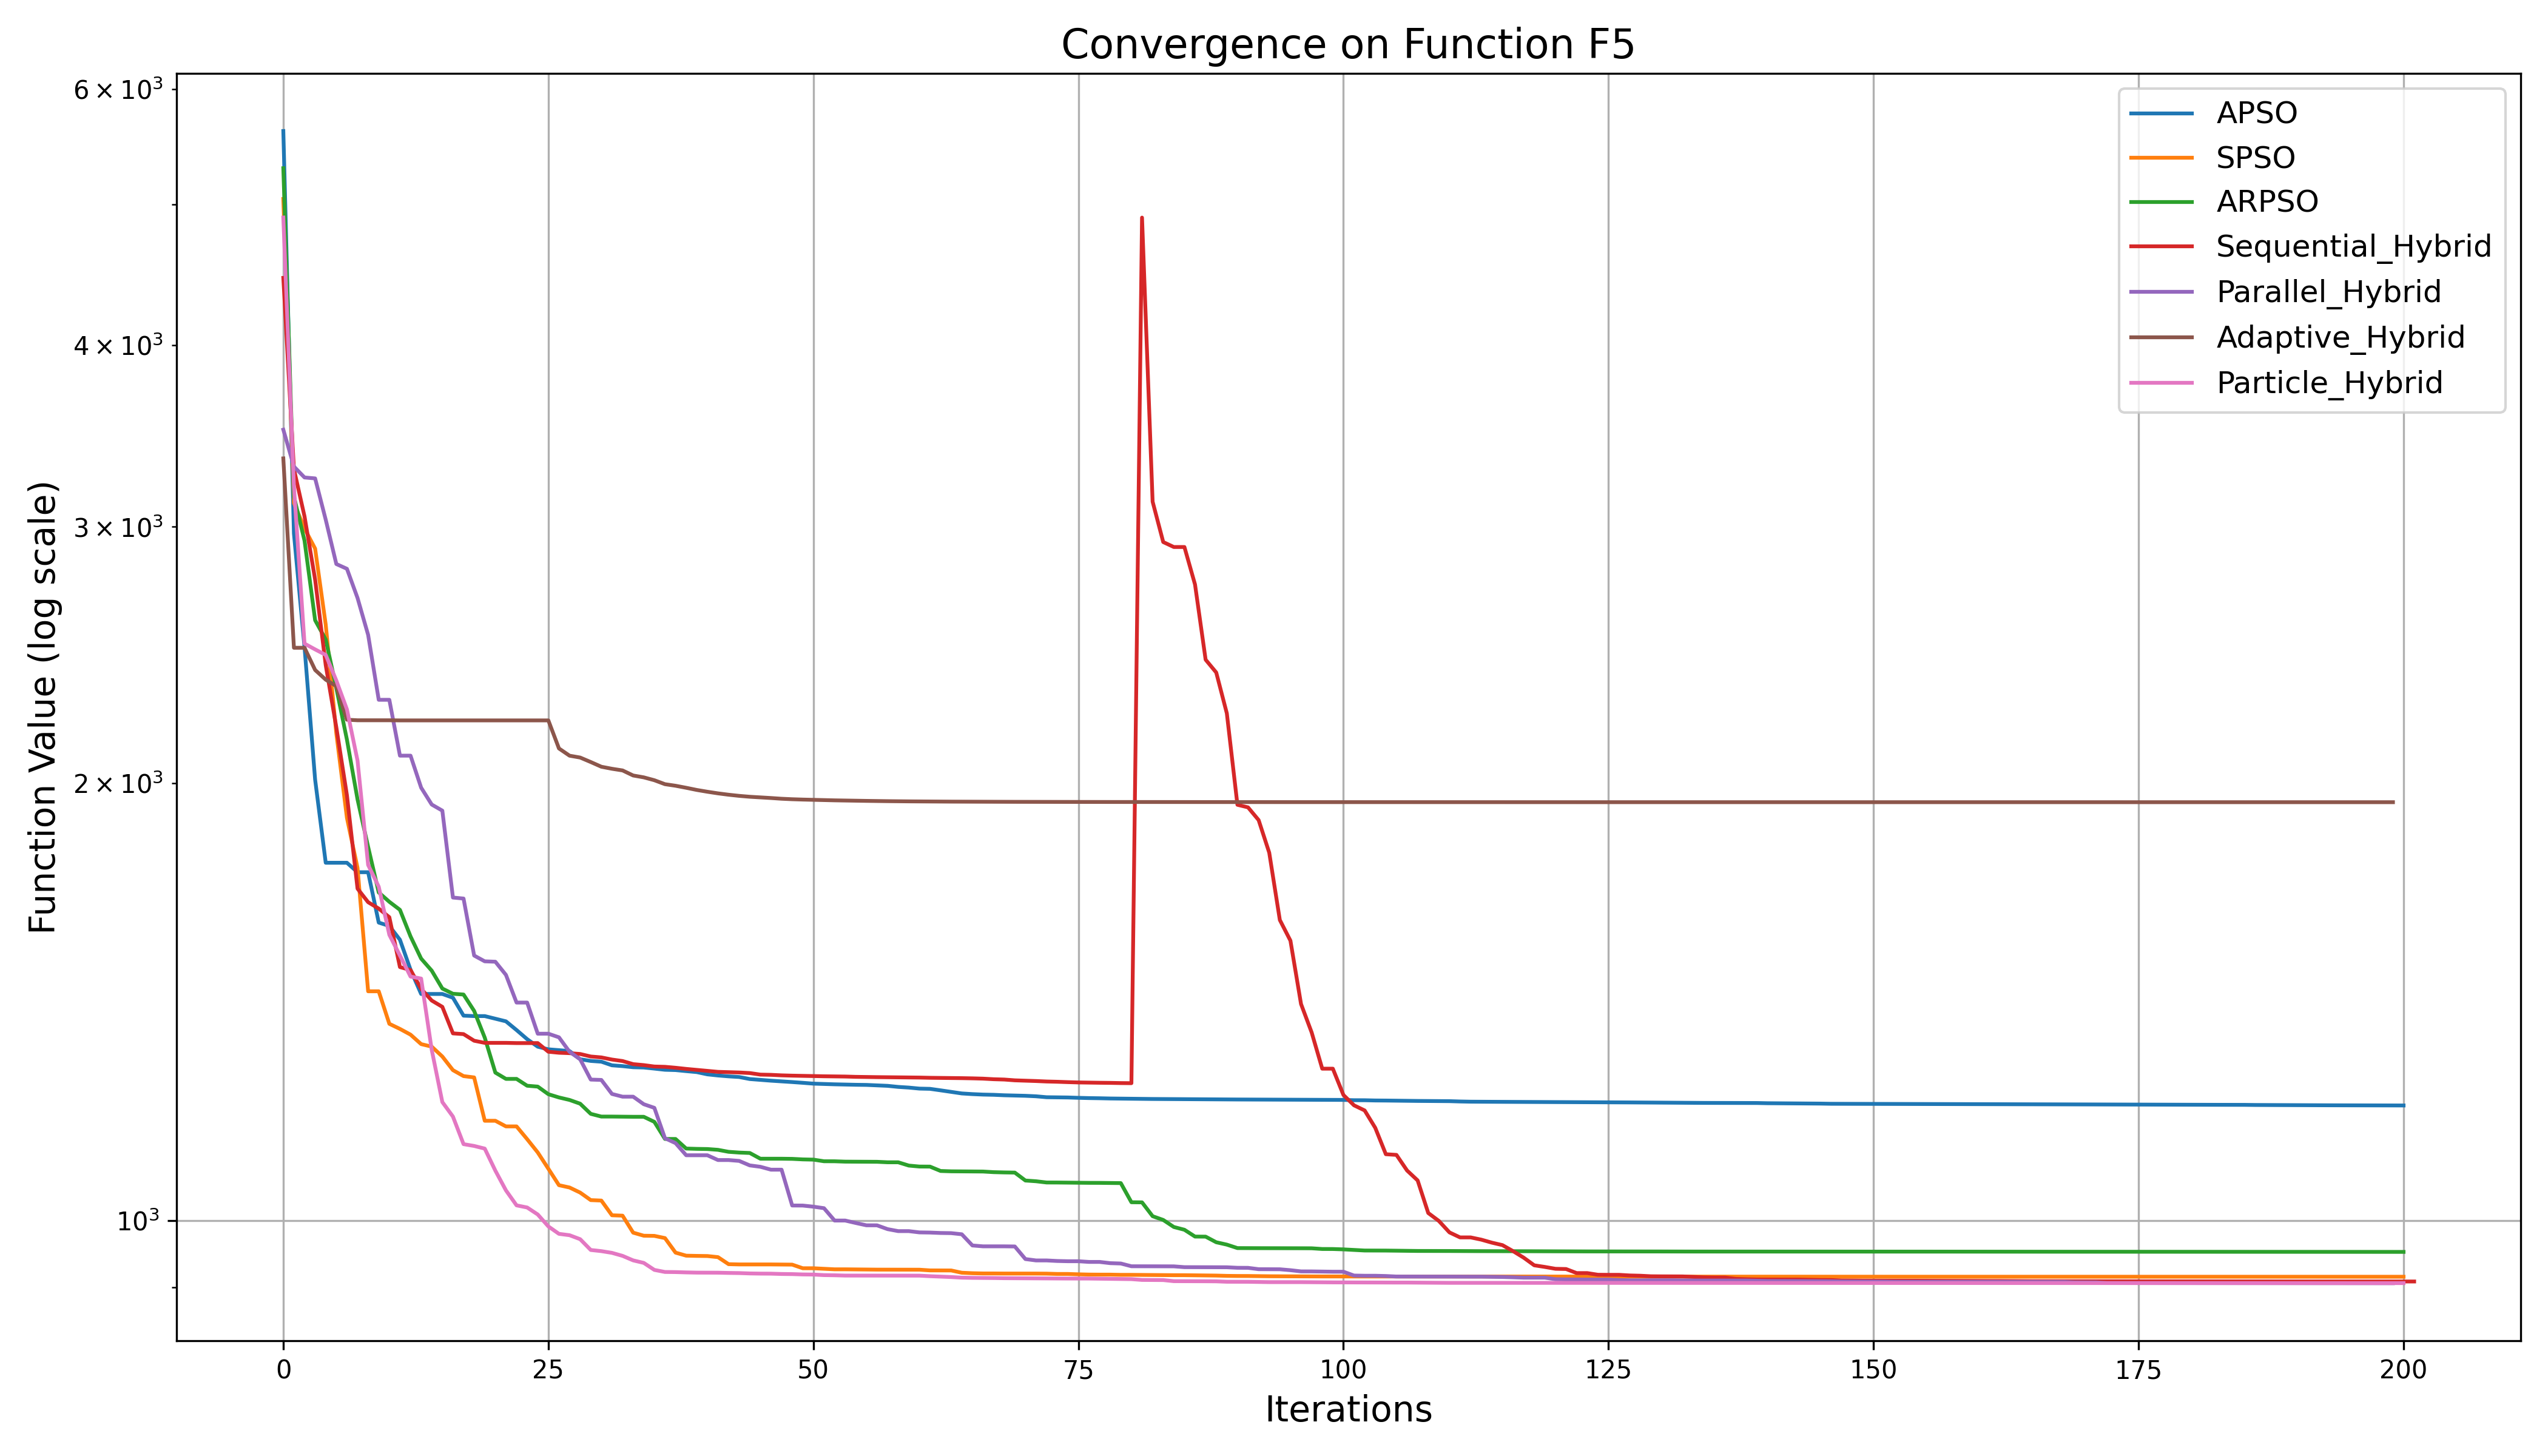
\includegraphics[width=\linewidth]{../plots/exploitation/hybrid_convergence_f5.png}
    \caption{F5 (Levy)}
    \label{fig:hybrid_conv_f5}
\end{subfigure}

\caption{Convergence plots for hybrid approaches on CEC 2022 benchmark functions}
\label{fig:hybrid_convergence}
\end{figure}

Table \ref{tab:hybrid_results} summarizes the performance ranking of all algorithms across the five benchmark functions, with 1 indicating the best performance and 7 the worst.

\begin{table}[htbp]
\caption{Performance Ranking of Algorithms (1=Best, 7=Worst)}
\begin{center}
\begin{tabular}{|c|c|c|c|c|c|c|c|}
\hline
\textbf{Algorithm} & \textbf{F1} & \textbf{F2} & \textbf{F3} & \textbf{F4} & \textbf{F5} & \textbf{Wins} & \textbf{Avg Rank} \\
\hline
Particle\_Hybrid & 1 & 4 & 3 & 5 & 3 & 1 & 2.20 \\
\hline
Parallel\_Hybrid & 6 & 3 & 1 & 4 & 1 & 2 & 3.20 \\
\hline
APSO & 2 & 2 & 2 & 2 & 7 & 0 & 3.60 \\
\hline
SPSO & 3 & 5 & 4 & 1 & 5 & 1 & 3.60 \\
\hline
Sequential\_Hybrid & 5 & 6 & 5 & 3 & 2 & 0 & 4.00 \\
\hline
ARPSO & 4 & 1 & 6 & 6 & 6 & 1 & 4.80 \\
\hline
Adaptive\_Hybrid & 7 & 7 & 7 & 7 & 4 & 0 & 6.60 \\
\hline
\end{tabular}
\label{tab:hybrid_results}
\end{center}
\end{table}

\subsection{Discussion}
The hybrid approaches show interesting performance patterns:

\begin{itemize}
    \item Particle Hybrid performs well overall (average rank 2.2)
    \item Sequential Hybrid shows mixed performance (average rank 4.0), with a notable spike in the convergence plot at the transition point between APSO and SPSO phases
    \item Parallel Hybrid performs well overall (average rank 3.20), coming in second to Particle Hybrid (average rank 2.20)
    \item Adaptive Hybrid performs poorly (average rank 6.6), suggesting that frequent algorithm switching disrupts the optimization process
\end{itemize}

The strong performance of the Particle Hybrid approach suggests that combining different PSO variants within a single swarm allows the algorithm to leverage the complementary strengths of each variant. The particles using APSO dynamics can provide quick initial progress, while those using SPSO can refine solutions more precisely.

The poor performance of the Adaptive Hybrid approach is somewhat surprising but can be explained by several factors:
\begin{itemize}
    \item The 10-iteration evaluation window may be too short to accurately assess algorithm performance
    \item Frequent switching between algorithms disrupts the momentum and learning history of each method
    \item The performance metric (improvement in best solution) may not capture long-term potential
\end{itemize}

The spike in the Sequential Hybrid's convergence plot occurs at the transition point (around iteration 80) when the algorithm switches from APSO to SPSO. This happens because SPSO is initialized around APSO's final solution but with some random perturbation to maintain diversity. This perturbation temporarily worsens the fitness before SPSO begins to improve it. Reducing this perturbation could potentially eliminate this spike and improve overall performance.

\section{Conclusion and Future Work}
\subsection{Conclusion}
This report has investigated the performance of three PSO variants (SPSO, APSO, and ARPSO) in multi-UAV source seeking and optimization tasks, as well as four hybrid approaches that combine these variants.

Key findings include:

\begin{itemize}
    \item APSO consistently outperforms other variants in source seeking tasks, particularly in noisy environments, due to its second-order dynamics that provide smoother trajectories and better noise resilience
    \item SPSO shows superior performance on most benchmark optimization functions, demonstrating a better balance between exploration and exploitation for diverse optimization challenges
    \item ARPSO generally underperforms in both source seeking and benchmark optimization, though it occasionally excels on specific functions
    \item Among the hybrid approaches, Particle Hybrid shows the most promising overall performance, suggesting that combining different PSO variants within a single swarm can leverage their complementary strengths
    \item The performance of each PSO variant is strongly influenced by how well its movement dynamics match the characteristics of the problem landscape
\end{itemize}

These results provide valuable insights for algorithm selection in multi-UAV applications and suggest that hybrid approaches can offer performance improvements over individual PSO variants.

\subsection{Future Work}

\begin{itemize}
    \item Conduct more extensive experiments (10-30 runs) to ensure statistical significance of the results
    \item Refine the Sequential Hybrid approach by reducing or removing random perturbation during the transition between algorithms
\end{itemize}

By addressing these areas, we aim to develop more robust and efficient algorithms for multi-UAV coordination in complex environments.

\begin{thebibliography}{00}
\bibitem{10312321} A. Shankar, Himanshu, H. Kandath, and J. Senthilnath, "Acceleration-Based PSO for Multi-UAV Source-Seeking," in IECON 2023- 49th Annual Conference of the IEEE Industrial Electronics Society, pp. 1-6, 2023, doi: 10.1109/IECON51785.2023.10312321.
\bibitem{luo2022benchmarkfunctionscec2022} W. Luo, X. Lin, C. Li, S. Yang, and Y. Shi, "Benchmark Functions for CEC 2022 Competition on Seeking Multiple Optima in Dynamic Environments," arXiv preprint arXiv:2201.00523, 2022. [Online]. Available: https://arxiv.org/abs/2201.00523
\end{thebibliography}

\end{document}